\chapter{Forschungsmethoden}
	\abschnittsautor{F. Schäfer, M. Trognitz}
	\label{methoden}
Die Ergebnisse aus verschiedenen in den Altertumswissenschaften angewandten Methoden setzen sich oft aus mehreren verschiedenen Dateien unterschiedlicher Formate zusammen. Dadurch gehen die Ansprüche an die Dokumentation und die erforderlichen Metadaten zu den einzelnen Dateiformaten über die des Kapitels zu Dateiformaten hinaus und unterscheiden sich von Methode zu Methode. 

Sofern spezifische Dateiformate eine besondere Relevanz besitzen, sind diese entweder hier beschrieben oder es wird auf die entsprechenden Abschnitte im Kapitel Dateiformate auf Seite \pageref{dateiformate} verwiesen.

Da die Kapitel der einzelnen Forschungsmethoden von verschiedenen Spezialisten verfasst wurden, können sie deshalb und in Abhängigkeit von der jeweils beschriebenen Methode in Inhalt, Länge und Gliederung sehr unterschiedlich ausfallen.

Die vorhandenen Inhalte decken nur einen kleinen Teil der angewandten Forschungsmethoden in den Archäologien und Altertumswissenschaften ab. Weitere Inhalte sind geplant, wobei dafür auch Autoren gesucht werden. Die folgende Auflistung soll einen Eindruck der möglichen Inhalte vermitteln, wobei weitere Vorschläge und Ergänzungen willkommen sind.

3D-Scanning · Anthropologie · Archäobotanik · Archäometrie · Archäozoologie · Ausgrabung · Bauforschung · Datierungsmethoden · Geoarchäologie · Numismatik · Oberflächenbegehung (Survey) · RTI · Textanalyse

Bis wir Ihnen ausführlichere Hinweise zur Verfügung stellen können, können Sie sich auf den Seiten des \href{http://guides.archaeologydataservice.ac.uk/g2gp}{Archaeology Data Service informieren}, wo insbesondere folgende Inhalte zu Forschungsmethoden zur Verfügung stehen.

Dendrochronolgie $\cdot$ Fernerkundung $\cdot$ GIS $\cdot$ Geophysik $\cdot$ Laserscanning $\cdot$ Photogrammetrie $\cdot$ UAV Survey $\cdot$ Unterwassersurvey

\section{Geodäsie}
\abschnittsautor{K. Heine, U. Kapp}
Bitte beachten Sie, dass die Inhalte dieses Abschnittes den Inhalten des IT-Leitfadens des DAIs von 2011 entsprechen.
\begin{center}
\tib{\rule{0.9\textwidth}{0.2mm}}\vspace{3mm}
\end{center}
Alle Protokolle von Messungsrohdaten, mit Ergebnissen der Netzmessungen, der Ausgleichung und Festpunktkoordinaten inkl. Einmessungsskizzen müssen im \gls{ASCII}-Format (\gls{TXT}, \gls{CSV}, DAT) gespeichert werden.
	\subsection*{Vermessungswesen}
Es ist ja eine Binsenweisheit, dass archäologische und bauforscherische Tätigkeiten nicht ohne fundierte vermessungstechnische Basis- und begleitende Arbeiten auskommen. Die Zeiten, in denen man im 5X5 Meter Planquadrat seine Erkenntnisse sammelte, gehören zwar nicht der Vergangenheit an, aber die Bedingung ist, dieses Planquadrat in einen globalen Zusammenhang zu bringen. Die Vermessung bekommt in diesem Fall eine andere Bedeutung, die von der bloßen Herstellung von rechtwinkligen Quadranten abweicht. Andere Unterlagen wie Satelliten Images und Luftbilder sowie genaueres Kartenmaterial oder auch Unterlagen von z. B. geomagnetischen Prospektionen geben der Vermessung eine neue Wertigkeit.

Aber: der Einsatz elektronischer und satellitengestützter Geräte führt leider wie auch in der digitalen Fotografie zu einer fast unkontrollierbaren Anhäufung von Daten. Diese Ergebnisse müssen kurz-und langfristig verwaltbar sein. Aber dafür gibt es keine Ideallösung, weil die Entwicklungen im Gerätebau und den damit zusammenhängenden Programmen sich überschlagen, und was heute noch als Standard gilt, ist morgen schon überholt.

Meine Empfehlung: die Ergebnisse möglichst schnell auswerten, solange sie noch lesbar sind, denn nach wie vor ist eine Langzeitarchivierung von digitalen Daten nicht gesichert.

\subsubsection*{Bezugssystem für Messdaten}
Nach wie vor ist für viele archäologische Aktivitäten die Vermessungsgrundlage ein lokales Vermessungsnetz, das nicht in überörtliche oder gar in globale Systeme eingebunden ist. Für kleinere Messgebiete ist das legitim, solange sie nicht in einen Zusammenhang gebracht werden müssen.

Da das DAI aber in der Zwischenzeit viele Projekte mit großer räumlicher Ausdehnung bearbeitet, ist es sinnvoll, Messdaten in globalen Systemen zu erfassen, was durch die mittlerweile zur Verfügung stehenden Methoden und Geräte der Satelliten gestützten Vermessung deutlich vereinfacht wird. Durch die Einbeziehung von GPS-Messungen (Genauigkeit 5-10 m) und Differential GPS-Messungen (Zentimetergenauigkeit) kann der räumliche Zusammenhang von verschiedenen Arbeitsplätzen hergestellt werden.

Als Voraussetzungen für globale Positionierungsbestimmungen mit cm-Genauigkeit muss entweder ein Punkt im globalen Koordinatensystem (im Umkreis von 10 km) bekannt sein oder die Möglichkeit der Einbindung eines Satellitenpositionierungs-services (z. B. EGNOS) bestehen. Eine hinreichende Genauigkeit kann auch erzielt werden, wenn auf einem Punkt im Messgebiet entsprechend lange Beobachtungszeiten registriert werden. Grundsätzlich sollten für die Anlage von Vermessungsnetzen im globalen Koordinatensystem mittels GPS Zweifrequenzempfänger benutzt werden. Alternativ können Einfrequenzempfänger mit langer Beobachtungszeit (mindestens 20 min) genutzt werden. Eine Netzauswertung sollte im Post Processing erfolgen. Für die Ermittlung von Höhen sind ein Referenzpunkt sowie ein Geoid-Modell notwendig.

\subsubsection*{Geografisches System}
Grundsätzlich sollte als geografisches Bezugssystem das System WGS 84 (World Geodetic System 84) gewählt werden. Dieses ist auch Bezugssystem für das Satellitennavigationssystem GPS und zukünftig auch für das europäische System Galileo. WGS 84 ist ein räumliches, globales, geozentrisches System mit den rechtwinkligen Koordinaten x,y,z oder wahlweise auch geografischen Koordinaten geografische Länge (longitude) L und geografische Breite (latitude) B (\textdegree,',''). Die Koordinaten lassen sich nach Bedarf in andere Koordinatensysteme transformieren.

\subsubsection*{Geodätisches System}
Für praktische Zwecke der Aufnahme mit der Totalstation und Darstellung von Objekten in Zeichnungen und Plänen, insbesondere für großmaßstäbige Darstellungen (großmaßstäbig bedeutet hier: großer Abbildungsmaßstab, demzufolge i.d.R. kleineres Gebiet) ist dieses räumliche System in ein Abbildungssystem (geodätisches Koordinatensystem, projected coordinate system) zu transformieren. Hierfür eignen sich insbesondere transversale Zylinderabbildungen wie die UTM-Abbildung (Universal Transversal Mercator projection). Mit der UTM-Abbildung können auch lokale Systeme realisiert werden, indem als Mittelmeridian (central meridian) ein durch das Aufnahmegebiet verlaufender Meridian (Längengrad) und als Maßstab der Wert 1,0000 festgelegt wird. Die Angabe der UTM-Koordinaten erfolgt als East (E)- und North (N) - Wert.

\subsubsection*{Nationale Systeme}
In vielen Ländern existieren ein oder mehrere amtliche Systeme, denen unterschiedliche Bezugsellipsoide (z.B. Hayford, Bessel, Krassowski o.a) mit unterschiedlichem Datum (Lagerung) und verschiedene Abbildungsmethoden (stereografisch, Lambert, Gauß-Krüger, UTM o.a.) zugrundeliegen. Sofern Ellipsoidparameter, Lagerung und Abbildungsverfahren bekannt sind, kann auch in diesen Systemen gearbeitet werden, da diese dann jederzeit in andere Systeme transformierbar sind. Sofern die Parameter nicht bekannt sind, ist zu empfehlen, ein eigenes System unter Verwendung des WGS 84 und der UTM-Abbildung (s.o.) zu wählen und bestehende Karten im unbekannten System über Passpunkte in das neue System zu integrieren.

Momentan verfügen die meisten europäischen Staaten und auch die meisten Bundesländer noch über eigene amtliche Systeme. Für die nächsten Jahre ist aber der Übergang zum einheitlichen System ETRS89 (European Terrestrial Reference System 89) geplant. ETRS89 basiert auf dem Ellipsoid GRS80 (für praktische Zwecke mit WGS 84 identisch) sowie der europäischen Lagerung ETRF (European Terrestrial Reference Frame) von 1989. Als Abbildungsverfahren wird die UTM-Abbildung mit $6^{\circ}$ Streifenbreite und dem Maßstabsfaktor 0.9996 gewählt. Messungen in Deutschland sowie in den betroffenen europäischen Staaten sollten dann grundsätzlich ebenfalls in diesem System erfolgen, da die amtlichen Koordinaten für Festpunkte sowie Geobasisdaten dann ebenfalls in diesem System vorliegen.

\subsubsection*{EPSG}
International werden Bezugssysteme nach dem System der EPSG (European Petroleum Survey Group) angegeben. Die EPSG stellt die Parameter für die meisten Bezugssysteme bereit. Diese sind als Download auf den Webseiten der EPSG (www.epsg.org) zu beziehen.

\subsubsection*{Örtliche Systeme für die Bauforschung}
In der Bauforschung ist auch ein objektbezogenes Koordinatensystem, welches beispielsweise parallel zur längsten Bauwerksachse ausgerichtet ist und einen beliebigen Koordinatenursprung besitzt, anwendbar. Dies ist für große und komplexe Bauwerke unter Umständen praktikabler als die Verwendung eines globalen Systems. Um die Messungen bzw. Pläne später in solch ein übergeordnetes System einhängen zu können, sollten mindestens drei Passpunkte bestimmt werden, deren Koordinaten sowohl im bauwerksbezogenen, als auch im globalen System (bestimmbar beispielsweise mittels GPS) bekannt sind.

\subsection*{Einsatz von Hard- und Software in der Praxis}
Da es eigentlich nur noch zwei wesentliche Hersteller von Vermessungsgeräten gibt - Leica und Trimble, die alle anderen Hersteller integriert haben - liegt der Entschluss, welches Gerät man wählt, eigentlich nur in der Beziehung, die zum Verkäufer besteht, denn preislich findet man die Unterschiede nicht mehr so groß. Auch die Handhabung ist nicht so unterschiedlich, da sie einem Schema folgt: Gerät aufbauen, Orientieren, Messen, Auslesen. Bei Neuanschaffungen sollte darauf geachtet werden, dass eine Systemreihe fortgeführt wird, wenn nicht zwingende Gründe dagegen sprechen, denn mit jedem Gerätesystemwechsel geht auch ein Softwarewechsel einher.

Eine Beschreibung der Handhabung der Geräte geht meistens aus der Gebrauchsanleitung hervor und würde den Rahmen dieses Leitfadens sprengen.

\subsubsection*{Messungsdaten}
Ich möchte hier nicht das Handaufmaß einbeziehen, sondern nur die elektronischen Messweisen mit Totalstation und GPS. Laserscan-Daten fallen beim DAI noch nicht an, da es noch kein eigenes Gerät gibt. Zum Handaufmaß gehören auch Daten, die mit Laser-Distomat gemessen, also nicht registriert, gespeichert werden.

Grundsätzlich muss man die eigentliche Vermessung von der Weiterverarbeitung im Computer trennen, da es für viele Vermessungsgeräte nach wie vor keine direkte Schnittstelle zum Computer gibt, sieht man von einigen Programmen ab, wie z.B. TachyCad als Aufsatz für AutoCad. Doch damit tauchen dann auch andere Probleme auf, die hardwaremäßig bedingt sind.

Sämtliche Vermessungsdaten der gängigen Totalstationen lassen sich mit den vom Hersteller des Geräts beigefügten Programmen in \gls{ASCII}, \gls{TXT}- oder \gls{DXF}-Dateien in den Computer übertragen. Für die Weiterverarbeitung in CAD-Programmen bedarf es nun eines Transferprogramms, damit -- besonders bei AutoCad -- diese Daten erkannt und als Objekte behandelt werden können.

Es gibt einige Profi-Programme. Ich benutze seit Jahren BB-VermCad und bin, auch weil ich es gut kenne, damit zufrieden. Nur hat es, wie jedes Aufsatzprogramm den Nachteil, dass vorhandene Versionen nie kompatibel mit neueren Versionen von AutoCad sind, man also theoretisch mit jeder neueren Ausgabe von AutoCad auch eine neue Version von BB kaufen müsste; oder man behält die laufende Version - auch von AutoCad - zur Bearbeitung der Vermessungsdaten auf dem Rechner und lädt dann die erhaltenen Ergebnisse in die neue Version. Die Frage ist, ob man diese neuen Versionen braucht? Meine Antwort: leider ja, da viele Kollegen sich diesem Trend nicht ausschließen, und dann plötzlich Ergebnisse im Austausch nicht mehr kompatibel sind, weil sie mit verschiedenen Versionen abgespeichert wurden (down-kompatibel ist fast immer möglich, up-kompatibel fast nie!).

AutoCad, MicroStation, ArchiCad sind nur drei Programme, die mir im Laufe meines Arbeitslebens als Vermesser begegnet sind. Von diesen ist AutoCad am verbreitetsten, und zusätzliche Programme (BB, TachyCad) werden auch nur für ACAD gemacht. Auch "`handgeschriebene"' Programme beziehen sich fast nur auf ACAD, da AutoCad eine eigene Programmiersprache\footnote{AutoCad lisp (*.lsp)}, die relativ leicht zu erlernen sein soll, beinhaltet. Es ist nicht nur eine Sache des guten Geschmacks sondern auch eine Antwort auf die Frage: welches Programm benutzt mein Kollege, und der Kompromiss ist AutoCad.

Das einzige Austauschformat zwischen unterschiedlichen Programmen - *.dxf - ist hier mit Vorsicht zu genießen, da es auch versionsabhängig ist. Häufig wird die gesamte *.dxf-Datei nicht von einem anderen Programm vollständig gelesen, besonders bei 3D-Dateien kann es hier zu Irritationen führen.

Es gilt also, einen Standard aufzubauen, der sowohl Geräte als auch Computerprogramme einschließt.

\subsubsection*{Netzmessungen}
Eine dauerhafte Sicherung der Messungsrohdaten scheint nur für die Vermessung der Grundlagennetze sinnvoll. Dies gilt sowohl für terrestrische als auch für GPS-Messungen. Für jedes Projekt sollten die Festpunktkoordinaten und die Festpunktbeschreibungen inkl. der Einmessungsskizzen gespeichert werden.

\subsubsection*{Objektpunkte}
Ob es sinnvoll ist, die Koordinaten aller aufgemessenen Punkte dauerhaft zu sichern ist fraglich, denn entweder werden bei der Aufmessung alle relevanten Informationen zu einem Punkt mit eingegeben (was sehr aufwendig ist) und abgespeichert, oder es muss, um die Messung nachvollziehen zu können eine eindeutige Skizze (Feldriss) vorhanden sein, die dann ebenfalls dauerhaft (digitalisiert) gespeichert werden müsste.

Wenn eine dauerhafte Sicherung erfolgen soll, sollte dies im ASCII-Daten-Format (*.txt, *.dat, *.csv o.ä.) erfolgen, da die meisten CAD-Programme diese in irgendeiner Form erkennen. Häufig müssen die Daten mit Zusatzprogrammen (s.o.) CAD-gerecht aufbereitet werden. Es gibt in diesem Fall auch keine Empfehlung, da die Programme nur bedingt kompatibel sind. Wie schon erwähnt, ist auch das *.dxf-Format nur mit Vorsicht zu benutzen, EXCEL-Dateien müssen auch wieder in *.txt-Dateien gespeichert werden, usw.

Man erreicht einen Standard nur dann, wenn alle Beteiligten die gleichen Programme der gleichen Version benutzen.

Um Zeichendateien, bei AutoCad *.dwg auszutauschen, empfehle ich die Dateien in einer Version (2000, 2002) abzuspeichern, die ohne Schwierigkeiten und Verluste auch mit einer neueren Version zu öffnen ist. Die meisten 3D-Daten lassen sich so verlustfrei austauschen.

\subsection*{Quellen}
\begin{flushleft}
Bauer, M.: Vermessung und Ortung mit Satelliten. Wichmann Verlag Heidelberg

Schimke, A.: Kartenprojektionen und Koordinatentransformationen

Zeiske, K.: Vermessen leicht gemacht. Leica Publikation

Herrmann K.: Bautechnische Vermessung. Dümmlers Verlag Bonn

Seckel/Hell/Schnuchel: Vermessungskunde und Bauaufnahme für Architekten. Herbert Wichmann Verlag Karlsruhe

GPS Basics, Einführung in die GPS Vermessung, Leica Publikation

Gebrauchsanweisungen für Geräte beinhalten häufig gute Ratschläge

\url{http://www.olanis.de/knowhow/mapprj/index.shtml}

\url{www.epsg.org}
\end{flushleft}

%%%%%%%%%%%%%%%%%%%%%
%% Alte Gliederung %%
%%%%%%%%%%%%%%%%%%%%%
%\subsection{Terrestrische Messungen}
%\subsubsection{GPS/GNSS}
%\subsubsection{Photogrammetrie}
%\subsubsection{Tachymetrie}
%\subsubsection{Terrestrisches Laserscanning}

%\subsection{Fernerkundung}
%\subsubsection{LIDAR-Geländescans}
%\subsubsection{Luftbild}
%\subsubsection{Luftbildphotogrammetrie}

\section{Georeferenzierung}
\abschnittsautor{K. Heine, U. Kapp}
	%
% Georeferenzierung
%
Bitte beachten Sie, dass die Inhalte dieses Abschnittes den Inhalten des IT-Leitfadens des DAIs von 2011 entsprechen.
\begin{center}
\tib{\rule{0.9\textwidth}{0.2mm}}\vspace{3mm}
\end{center}

GeoReferenzierung, d.h. Zuordnung von Koordinaten zu Bildpunkten auf Fotos und Plänen (Karten), die in Digitaler Form vorliegen.
Mit der GeoReferenzierung erreicht man gleichzeitig eine Entzerrung dieser Grundlagen. Vorbedingung ist ein Programm, mit dem man diese Arbeit durchführen kann. Jedes GIS (Geoinformationssystem) hat notwendigerweise ein Modul für GeoReferenzierung.

\paragraph{Einsatz von Hard- und Software in der Praxis}
Die GeoReferenzierung von Topographischen Karten ist in der Regel einfach, da Koordinaten normalerweise in Form eines Rasters auf den Karten vorhanden sind. Es wird komplizierter, wenn man mit diesen Koordinaten nicht arbeiten möchte. Dann wird es erforderlich, entweder vor Ort Vergleichspunkte (Referenzpunkte) zu messen oder mit anderen Programmen die vorhandenen Koordinaten in das gewünschte System zu transformieren. Viele GIS-Programme erlauben auch das. Ich habe Erfahrungen mit dem einfachen FUGAWI, das für die Bearbeitung der GPS-Daten der Handgeräte vorhanden ist.

Eine andere Möglichkeit, Referenzpunkte zu bekommen, bildet im Moment GOOGLE EARTH.  Besonders in den Bereichen mit hoher Auflösung bekommt man eine ausreichend genaue Informationen. Zu berücksichtigen ist natürlich der Maßstab, in dem man später arbeiten möchte. 

Die Anzahl der Referenzpunkte richtet sich nach dem Inhalt des Images. Liegt eine flächenfüllende Karte vor, reichen mindestens 4 Punkte in den Ecken der Karte. Zu empfehlen sind Kontrollpunkte; bei einer Karte würde ich die doppelte Anzahl an Punkten wählen, um auch bei der Entzerrung sicher zu sein.

Bei Fotos, die kein Raster vorgegeben haben, muss man daher mehr Punkte wählen, die das Foto bis an die Ränder der Darstellung bearbeiten können oder beschneidet das Image auf die Größe , die benötigt wird. Die Punkte bezieht man aus Messungen vor Ort oder aus einer Karte oder anderen Medien (GOOGLE EARTH). Es müssen auch Punkte innerhalb des Images bestimmt werden, um die Kontrolle über das Bild zu erhalten. 4 Punkte sind da nicht ausreichend, ich empfehle die doppelte Anzahl. Das richtet sich nach der Geometrie des Fotos.

Wenn verfügbar, sollten digitale Orthophotos bzw. Luftbildkarten an Stelle von Luftbildern verwendet werden, da diese bereits auf ein digitales Geländemodell entzerrt sind. Bei ebenem Gelände kann eine Entzerrung gemäß Tabelle 1 vorgenommen werden, ohne dass dabei größere Lageungenauigkeiten  hervorgerufen werden. Durch eine Entzerrung von Luftbildern von unebenem Gelände mit polynomialen Ansätzen höherer Ordnung können keine Unstetigkeiten im Gelände wie beispielsweise steile Felshänge o.ä. berücksichtigt werden. Hier ist eine Entzerrung auf ein digitales Geländemodell vorzunehmen (s. Tab. 1).

Natürlich mangelt es auch hier nicht an Programmen, die diese Arbeiten durchführen können. Jedes GIS Programm hat ein Modul für die Georeferenzierung von Rasterdaten. Die Ergebnisse sind untereinander austauschbar, da das gleiche Dateiformat benutzt werden kann. Man kann also ein "`world-tiff oder jpg"` in ein anderes GIS Programm exportieren. 

AutoCad Map oder der AutoCad Aufsatz PhoToPlan bieten auch die Möglichkeit der Affinen Transformation oder sogar der Polynominalen Entzerrung. Leider sind die neu entstandenen Rasterdaten nur in diesen Programmen verwendbar. Beim Export dieser Rasterdaten in GIS Programme müssen sie wieder neu referenziert werden.

Auch bei Anwendung der Digitalen Bildentzerrung bei der Bauaufnahme oder bei Grabungsflächen oder Grabungsprofilen kann eine Georeferenzierung durchgeführt werden. Die Referenzpunkte müssen eingemessen werden, wobei darauf zu achten ist, dass die Digitale Bildentzerrung nur 2-D einsetzbar ist. Um Strukturen mit unterschiedlicher Höhe mit diesem Verfahren zu bearbeiten, ist es notwendig, die Ebenen separat zu definieren und zu entzerren. PhoToPlan erlaubt die Montage eines Bildverbands, solange genügend verbindende Passpunkte vorhanden sind.


Die Tabelle mit der Übersicht der unterschiedlichen Entzerrungs-und Referenzierungsmethoden entnehmen Sie bitte Seite 28 des IT-Leitfadens des DAIs (\url{http://www.ianus-fdz.de/it-empfehlungen/sites/default/files/ianusFiles/IT-Leitfaden_Teil2_v100_DAI.pdf})


\paragraph{Quellen}
\begin{flushleft}
Alle Handbücher der GIS Programme, AutoCad Map, PhoToPlan etc. \urllist{http://www.giub.uni-bonn.de/gistutor/}
\end{flushleft}

\section{Oberflächen- (DOM) und Geländemodellierung (DGM)}
\abschnittsautor{K. Lambers, M. Reindel}
	%
% Oberflächenmodellierung
%
Bitte beachten Sie, dass die Inhalte dieses Abschnittes den Inhalten des IT-Leitfadens des DAIs von 2011 entsprechen.
\begin{center}
\tib{\rule{0.9\textwidth}{0.2mm}}\vspace{3mm}
\end{center}

Bei Geländemodellen ist zwischen primären und sekundären Geländemodellen zu unterscheiden:

a) primäre Geländemodelle

Aus Messung entstandene Geländemodelle sind über die Vermessungsdaten zu speichern.

b) sekundäre Geländemodelle

Aus primären Geländemodellen abgeleitete Geländemodelle (z.B. erworbene Geländemodelle) sind als Rasterdaten im TIFF-Format abzuspeichern.

\paragraph{Eine kurze Einführung}
Um Oberflächen maßstabsgetreu darstellen zu können, müssen sie vorher durch geeignete Vermessungen aufgenommen werden. Dies kann durch Handvermessung geschehen oder aber durch den Einsatz moderner Messinstrumente. Je nach Art und Größe des Untersuchungsobjektes kommen unterschiedliche Methoden und Techniken zur Anwendung. Die Dokumentation der Oberflächen all dieser Objekte erfolgt prinzipiell nach den gleichen Methoden. Die folgenden Ausführungen konzentrieren sich auf die Dokumentation und Darstellung von Geländeoberflächen.

Als Messinstrumente kommen für mittlere und große Objekte Theodolithen bzw. Tachymeter (mit elektronischer Distanzmessung) zum Einsatz. Moderne Messverfahren bedienen sich auch der Photogrammetrie (Vermessung in stereoskopisch aufgenommenen Bildern) und neuerdings des Laserscannings oder LIDAR (engl. light detection and ranging, s. u.). Allen Aufnahmeverfahren ist gemeinsam, dass sie Lagekoordinaten der vermessenen Objekte in einem zuvor definierten Vermessungssystem liefern. Für eine planimetrische Darstellung (ohne Höhenangaben) reichen Messwerte in X- und Y-Richtung aus. Sie ermöglichen zweidimensionale Darstellungen (2D). Will man jedoch die Oberfläche eines Objektes oder von Gelände räumlich darstellen, benötigt man auch die Höheninformation, das heißt einen Z-Wert. Die Grundlage einer räumlichen Darstellung einer Geländeoberfläche ist somit eine Sammlung von Punkten mit X-, Y- und Höheninformation in einem Koordinatensystem.

Im Gegensatz zu einer echten dreidimensionalen Darstellung (3D), in der X-, Y- und Höhenkoordinaten zu einem Volumenmodell verarbeitet werden, werden in sogenannten 2,5D-Darstellungen 2D-Daten mit einer zusätzlichen Höheninformationen versehen, die nicht als Koordinate, sondern als Attribut gespeichert wird. Dies bedeutet, dass jedem XY-Punkt nur ein Höhenwert Z zugeordnet werden kann, was die Modellierung von Senkrechten oder Überhängen ausschließt. Geoinformationssysteme, die ursprünglich für großflächige geographische Anwendungen entwickelt wurden, verarbeiten bis heute in der Regel nur 2,5D-Daten, während in CAD-Anwendungen, die für die Objektmodellierung entwickelt wurden, 3D-Informationen verwendet werden. Die Entwicklung geht jedoch in Richtung einer Konvergenz beider Systeme, so dass in Zukunft voll 3D-fähige GIS zum Standard werden dürften.

\subparagraph{Vermessung eines Grabungsgeländes}
Die Aufnahme von Messdaten mit dem Ziel, Gelände zu modellieren, spielt in der archäologischen Praxis zum einen bei der Dokumentation von Grabungsorten vor dem Beginn oder während der Ausgrabungen und zum anderen bei der Durchführung von Regionalstudien mit Hilfe von Geoinformationssystemen eine Rolle. Grabungsgelände werden in der Regel durch tachymetrische Vermessung aufgenommen, während die Topographie größerer Gebiete durch erworbene digitalen Kartendaten, Fernerkundungsdaten oder von Luftbildern erarbeitet wird.

Der erster Schritt bei der Vermessung eines Grabungsgeländes ist die Anlage eines Messnetzes. Dieses wird zumeist genordet, oft aber auch an den zu erwartenden Grabungsbefunden ausgerichtet. In der Regel wird zunächst ein Ausgangspunkt und eine Grundlinie angelegt und von dort das Messnetz aufgebaut. In anderen Fällen wird von dem Ausgangspunkt ein Polygonzug angelegt, von dem aus weitere Geländepunkte eingemessen werden.

Das Messnetz sollte an ein bestehendes übergeordnetes Messnetz angebunden werden. Bezugspunkte können vermarkte Messpunkte eines Landesvermessungsnetzes oder in abgelegeneren Regionen Triangulationspunkte von Kartierungsprojekten oder ähnliches sein. Die Koordinaten der Hauptmesspunkte können auch durch präzise GPS-Messungen bestimmt werden. Häufig werden bei der Anlage von Grabungen willkürliche Messpunkte festgelegt, die durch spätere Messungen an die übergeordneten Messnetze angebunden werden (siehe hierzu auch Kapitel 2).

Ausgehend von den Basispunkten des Messnetzes werden mit dem Tachymeter Geländepunkte aufgemessen. Bei der Auswahl der Punkte ist es wichtig sich zu vergegenwärtigen, welche Art und welcher Maßstab der Darstellung des Geländes angestrebt wird. Grundsätzlich sollten diejenigen Punkte aufgenommen werden, an denen sich die Geländeneigung oder der Verlauf einer gedachten Höhenlinie (Linie, die sich aus Punkten gleicher Höhe zusammensetzt) ändert. Das heißt, je unregelmäßiger die Geländeoberfläche ist und je detaillierter die Geländeoberfläche wiedergegeben werden soll, umso mehr Punkte pro gegebener Fläche sind aufzunehmen.

Die Punkte sind so dicht zu setzen, dass die relevanten Geländeformen in der graphischen Darstellung im angestrebten Maßstab wiedergegeben werden. Es ist einleuchtend, dass ein etwa 30 cm breiter Mauerzug, der sich im Gelände durch eine leichte Erhebung abzeichnet, nicht durch Punkte abgebildet werden kann, die im Abstand von 1 m gemessen wurden. Vielmehr muss zumindest der Beginn der Geländewölbung, der Scheitelpunkt über der Mauer und der Endpunkt der Geländewölbung vermessen werden. Bruchkanten müssen gesondert vermessen werden. Sie können bei der Auswertung der Messdaten mit Computerprogrammen speziell behandelt werden.

\subparagraph{Regionale Geländemodelle}
Ist das Untersuchungsgebiet größer als ein Grabungsgelände, werden dafür benötigte Geländemodelle üblicherweise nicht selbst erzeugt, sondern aus anderen Quellen erworben. Bezugsquellen für digitale Geländemodelle sind je nach Land staatliche Vermessungsämter, Universitäts- oder Forschungsinstitute für Geographie, Geodäsie, Kartographie oder Geophysik, Luft- und Raumfahrtagenturen oder das Militär.

Grundlage für die Erzeugung von Geländemodellen sind Fernerkundungsdaten, die entweder mit passiven Sensoren (Luft- und Satellitenbilder) oder mit aktiven Sensoren (Radar- oder Lidardaten) aufgenommen werden (siehe hierzu die Beiträge von Sabine Reinhold). Bilddaten werden mit photogrammetrischen Methoden ausgewertet. In überlappenden Bereichen benachbarter Bilder werden stereoskopisch homologe Punkte an der Erdoberfläche gemessen (engl. matching). Entweder werden ähnlich wie bei der terrestrischen Geländevermessung gezielt Einzelpunkte und ggfs. Bruchkanten gemessen, oder es werden bei automatisierten Verfahren Punkte in gleichmässigen Abständen gemessen. Photogrammetrische Auswertungen von Luftbildern bilden bis heute in vielen Ländern die Grundlage für die Produktion und Nachführung von topographischen Karten und für die Generierung von Geländemodellen.

Radar- und Lidardaten liefern demgegenüber direkte Informationen über die Distanz der gemessenen Punkte zum Sensor. Ein auf Radar (engl. radio detection and ranging) beruhendes Geländemodell der Shuttle Radar Topography Mission (SRTM) ist praktisch weltweit frei verfügbar und in vielen Gegenden die einfachste Möglichkeit, digitale Geländemodelle zu beziehen. Die geringe Auflösung von 90 m sowie Lücken und große Höhenfehler in gebirgigem Gelände sind jedoch limitierende Faktoren für die Verwendbarkeit. Vermessungen mit flugzeuggestütztem LIDAR (engl. light detection and ranging), bei dem die Erdoberfläche in hoher Dichte durch einen Laserstrahl gescannt wird, werden in Europa immer mehr zu einem Standardverfahren der Landesvermessung, sind jedoch in anderen Ländern oft noch nicht verfügbar.

Zur korrekten Georeferenzierung der Fernerkundungsdaten dienen GPS-Messungen, oft in einer Kombination von Positionsmessungen an Bord der Sensorplattform (z.B. GPS an Bord eines Flugzeuges gekoppelt mit INS, engl. inertial navigation system) mit Einmessungen von Kontrollpunkten am Boden, die in den Daten erkennbar sein müssen. Die GPS-Messungen dienen der Überführung der gemessenen Punkte von einem lokalen in ein globales Koordinatensystem (Georeferenzierung).

Erworbene Geländemodelle sind rechnerische Ableitungen von tatsächlich erhobenen Messdaten. Wie schon bei anderen Messdaten, sollten nach Möglichkeit auch die Rohdaten gespeichert werden. Beim Kauf von Standard-Produkten ist dies üblicherweise nicht möglich, wohl aber bei der Beauftragung von speziellen Geländemodellen, z.B. Lidar-Überfliegungen.

\subparagraph{Modellierung}
Zur Modellierung einer durchgehenden Oberfläche auf der Grundlage der vermessenen Punkte müssen die zwischen den Messpunkten liegenden Geländepunkte durch rechnerische Verfahren verknüpft werden. Dazu werden zunächst die Einzelpunkte zu einer aus Dreiecken bestehenden Oberfläche vermascht. Diese liegt im Vektorformat vor (engl. TIN: triangulated irregular network). Durch Interpolation werden die Vektordaten ggfs. in ein Rasterformat (z.B. Grid) mit einer festen Maschenweite überführt. Hierzu werden verschiedene mathematische Verfahren angewandt. Die Einzelheiten dieser Verfahren werden in den relevanten Computerprogrammen und Lehrbüchern erläutert, müssen jedoch vom Archäologen nicht im Detail nachvollzogen werden können. Wichtig ist jedoch, die Modellierungen mit den verschiedenen Verfahren zu testen, um entscheiden zu können, welche Methode die tatsächliche Geländeoberfläche am realistischsten darstellt. Die Maschenweite oder Zellengröße ist ein übliches Maß für die Auflösung eines Geländemodells. Während einige GIS-Programme (z.B. ArcGIS) auch TINs verarbeiten können, können viele andere nur mit Raster-Geländemodellen umgehen.

Je nach Platzierung der zu Grunde liegenden Messpunkte bilden Geländemodelle verschiedene Dinge ab. Als Oberbegriff dient die Bezeichnung Digitales Höhenmodell / DHM (engl. digital elevation model / DEM). Man unterscheidet zwei Typen von DHMs: 1. das Digitale Oberflächenmodell / DOM (engl. digital surface model / DSM), das die Erdoberfläche inklusive aller darauf befindlichen Objekte wie Häuser, Vegetation, etc. abbildet, und 2. das Digitale Geländemodell / DGM (engl. digital terrain model / DTM), das nur die Erdoberfläche abbildet. Bei der eigenen Vermessung des Grabungsgeländes wird man üblicherweise ein DGM erzeugen. Auch bei erworbenen Geländemodellen sind DGMs den DOMs vorzuziehen, da in archäologischen Untersuchungen üblicherweise die Geländegestalt ohne moderne Bebauung und Vegetation interessiert. Bei Geländemodellen mit geringer Auflösung wie dem SRTM-DHM sind die Unterschiede jedoch zu vernachlässigen.


\paragraph{Einsatz von Hard- und Software in der Praxis}
Für die Verarbeitung und die Interpolation der Messpunkte stehen unterschiedliche Computer-Programme zur Verfügung, darunter auch speziell auf die Messgeräte angepasste Software der Hersteller von Vermessungsgeräten (Zeiss, Leica, Wild, Sokkia, Trimble, etc.). In der archäologischen Praxis wird zur Verarbeitung und Umzeichnung von echten 3D-Messdaten zumeist das Programm AutoCAD verwendet (\url{http://www.autodesk.de}). Zur Generierung von Höhenlinien und 3D-Modellen können Zusatzmodule oder erweiterte Versionen erworben werden. Zur Modellierung von 2,5D-Geländeoberflächen kann auch jedes GIS-Programm verwendet werden.
Im Rahmen unserer Arbeiten wurden die Höhenlinien und Geländemodelle in der Regel mit dem Programm Surfer (\url{http://www.ssg-surfer.com/}) generiert. Surfer ist einfach zu handhaben und bietet eine Vielzahl von Möglichkeiten der Verarbeitung und Analyse archäologischer Daten. Unter anderem können auch Daten geophysikalischen Prospektionen einfach eingelesen und über die Geländemessdaten projiziert werden. Surfer ermöglicht auch die schnelle und einfache Überprüfung der Messergebnisse nach der Übertragung der Daten auf den Computer, wenn der Tachymeter nicht ohnehin mit einem Bildschirm ausgestattet ist. Die Koordinatenlisten lassen sich nachbearbeiten, Bruchkanten einfügen und nicht benötigte Messpunkte ausblenden. Die Höhenlinienpläne können als DXF-Dateien in AutoCAD exportiert werden. Schattierte oder farblich gestaltete Geländemodelle lassen sich in verschiedenen Graphikformaten (tiff, jpeg, bmp, etc.) exportieren und als solche ebenfalls in AutoCAD einbinden.

Erworbene Geländemodelle liegen üblicherweise in einem Rasterformat vor, in dem einer durch eine XY-Eckkoordinate definierten Zelle mit einer festgelegten Seitenlänge ein Höhenwert zugeordnet wird. Damit gleichen Raster-Geländemodelle im Prinzip Bilddaten, nur dass statt eines Farbwertes ein Höhenwert gespeichert wird. Deshalb können Geländemodelle z.B. auch als TIFF vorliegen. Ein anderes übliches Format ist ASCII; daneben gibt es proprietäre Formate wie z.B. ESRI Grid. Die Transformation von Raster-Geländemodellen von einem Format in ein anderes in einem GIS-Programm stellt üblicherweise kein unüberwindbares Problem dar, so dass hier kein Format empfohlen wird, zumal bei Standard-Produkten das Format oft bereits festgelegt ist.

Je nach gewähltem Ausgabemedium werden verschiedene Verfahren der Darstellung der Geländeoberflächen gewählt. Soll das Ergebnis auf Papier, also in 2D auf einem Plan als Arbeitsdokument oder für die Publikation ausgegeben werden, wird die Darstellung in Form von Höhenlinien, mit Schattierungen oder unterschiedlicher Farbgebung gewählt. AutoCAD-Dateien (*.dwg) lassen sich häufig nur mit Schwierigkeiten in andere vektorbasierte Programme (z.B. CorelDraw oder Adobe Illustrator) zur weiteren Bearbeitung exportieren. Für die Einbindung in Publikationen können AutoCAD-Pläne und -Zeichnungen jedoch als PDF-Dateien ausgegeben, in JPEG-Dateien umgewandelt und mit Bildbearbeitungsprogrammen ergänzt oder verändert werden. Am Computer können die räumlichen Modelle dargestellt, bewegt und von unterschiedlichen Standpunkten aus betrachtet werden.

GIS-Programme bieten die Möglichkeit, die in Geländemodellen enthaltene Höheninformation in verschiedener Form in 2D darzustellen, z.B. als Höhenlinien, Grauwerte oder Farbabstufungen. Das Layout von Karten ist in den verschiedenen Programmen unterschiedlich einfach zu handhaben, jedoch sind die grundlegenden Funktionen wie die automatische Platzierung eines Koordinatenrahmens, eines Maßstabes etc. überall vorhanden, so dass Karten im GIS-Programm erzeugt und entweder direkt ausgedruckt oder in ein Standard-Graphikformat (Vektor oder Raster) exportiert werden können.

\paragraph{Quellen}
\begin{flushleft}
Archaeology Data Service 2007: Guides to Good Practice. \urllist{http://ads.ahds.ac.uk/project/goodguides/g2gp.html}

Bill, Ralf 1999: Grundlagen der Geo-Informationssysteme, Band 2: Analysen, Anwendungen und neue Entwicklungen. 2. Aufl. Heidelberg: Wichmann. Kapitel 2.5: Digitales Geländemodell (DGM).

Conolly, James \& Mark Lake 2006: Geographical Information Systems in Archaeology (Cambridge Manuals in Archaeology). Cambridge: Cambridge University Press. Kapitel 6: Building Surface Models.

Howard, Phil 2007: Archaeological Surveying and Mapping: Recording and Depicting the Landscape. London: Routledge.

Wheatley, David \& Mark Gillings 2002: Spatial Technology and Archaeology: The Archaeological Applications of GIS. London: Taylor \& Francis. Kapitel 5: Digital Elevation Models.
\end{flushleft}

	
\section{Rekonstruktion}
\abschnittsautor{A. Müller, U. Wulf-Rheidt}
	%
% Rekonstruktion
%

%%%%%%%%%%%%%%%%%%%%%%%%%%%%%%%%%%%%%%%%%%%%%%%%%%%%%%%%%%%%%%%%%%%%%%%%%%%%%%%
%%DAI%%ALT%%DAI%%ALT%%ALT%%ALT%%ALT%%ALT%%ALT%%ALT%%ALT%%ALT%%ALT%%ALT%%ALT%%%%
%%%%%%%%%%%%%%%%%%%%%%%%%%%%%%%%%%%%%%%%%%%%%%%%%%%%%%%%%%%%%%%%%%%%%%%%%%%%%%%
Bitte beachten Sie, dass die Inhalte dieses Abschnittes den Inhalten des IT-Leitfadens des DAIs von 2011 entsprechen.
\begin{center}
\tib{\rule{0.9\textwidth}{0.2mm}}\vspace{3mm}
\end{center}

\paragraph{3D-Modelle}
Einfache 3D-Modelle sind relativ schnell angelegt und können zur visuellen Kommunikation einen erheblichen Beitrag leisten. Nach Auswertung erster Forschungs- oder Grabungsergebnisse entstehen oft erste, vereinfachte Massenmodelle, die z. B. der Erläuterung von Rekonstruktionsideen dienen können. Es ist dann kein Problem, die erstellten Volumina in georeferenzierte Systeme, wie beispielsweise Google Earth zu integrieren oder in präzisere Geländemodelle einzubauen. Im Verlaufe des Projektes wird das 3D-Modell in der Regel immer differenzierter ausgearbeitet und es werden mehr Datensätze und Informationen angehängt, in dem einzelne Gebäudeteile und Räume differenziert dargestellt, Bauteile ausgearbeitet, u.U. Bilder, Geodaten, Befund-Daten und Literaturhinweise angehängt und schließlich die zur Visualisierung notwendigen Texturen und Lichtquellen sowie dynamische und statische Schnitte generiert werden. Derart komplexe Aufgaben erfordern eine gut durchdachte Datenverwaltung, da ihr Verwaltungs- und Pflegeaufwand exponentiell zur Datenmenge anwächst. Deshalb ist es wichtig, sich vor Anlegen eines 3D-Modells über die Ziele, die verwirklicht werden sollen, klar zu werden. Wenn z.B. ein Modell nur benötigt wird, um einige Perspektiven für eine Publikation zu visualisieren, genügt es, die Kubatur des Gebäudes zu erstellen, sie zu texturieren, Lichtquellen zu setzen und Ansichtsdefinitionen festzulegen. Dementsprechend gering bleibt der Sicherungs- und Dokumentationsaufwand. Je genauer der Auftraggeber eines 3D-Modells die Ziele, zur Verwendung des Modells definiert, desto geringer kann der Aufwand der Datenerstellung und Datenhaltung gehalten werden. 

Deshalb sind Mindestanforderungen bei der Auftragsvergabe nur auf sehr niedrigem Niveau möglich. Zurzeit beschränken sich diese Forderungen in der Regel auf die Sicherung in einem gut dokumentierten Format wie z.B. dxf oder Wavefront OBJ-Dateien, mit allen Nachteilen, die sich dabei aus einer eventuellen Datenkonvertierung ergeben.

\paragraph{Praxis}
Es ist derzeit verbreitet, die Wahl der Software dem Zufall zu überlassen: Softwarekenntnisse des Bearbeiters, das Vorhandensein von Software oder die Frage, welche Software preiswert zu erwerben ist, bestimmen meist die Wahl.

Das bedeutet zwar nicht, dass eine spätere Entscheidung für eine andere Software zu totalem Datenverlust führen muss, denn grundsätzlich ist die Konvertierung beinahe jedes Zeichenformates in ein anderes möglich. Dies ist jedoch häufig mit erheblichen Informationsverlusten oder/und gewaltigem Arbeits- und Kostenaufwand verbunden.

Wurde ein Modell beispielsweise in einer Visualisierungssoftware wie Rhino, Maya oder 3ds Max erstellt, so haben die Objekte hauptsächlich Metainformationen hinsichtlich Geometrie und Textur. Mit dieser Software sind sehr hochwertige Bilder und Animationen generierbar, die Verwaltung hinsichtlich bautechnisch sinnvoller  Einheiten wie Wände und Fenster ist dagegen nicht vorgesehen und ist deshalb schwierig, zeitaufwändig und umständlich.

Architektursoftware bietet erhebliche Vorteile hinsichtlich der Datenverwaltung, da  Objekte von vornherein in üblichen Klassifizierungen, wie Wänden, Decken, Stützen, Böden und Öffnungen usw. verarbeitet werden können. Die Eingabe ist aufwändig, da sie parametrisch erfolgt. Sie bietet aber den Vorteil der Nachvollziehbarkeit. Außerdem besteht die Möglichkeit, zwischen verschiedenen Maßstäben hin- und herzuschalten und standardmäßig 2D-Schnitte und -Grundrisse darzustellen bzw. zu exportieren. Nachteile liegen vor allem im Preis der Anschaffung und der Notwendigkeit regelmäßig upzudaten, verlustfreier Datentransfer ist - wenn überhaupt - meist nur innerhalb der Produktgruppe des selben Software- Entwicklers möglich. Standardisierte Objekte wie Wände sind starr definiert und können nicht frei modelliert werden, eine verformungsgetreue Darstellung ist damit nicht möglich. Allerdings ist in den meisten Fällen eine verformungsgetreue Nachbildung des Baukörpers im Modell nicht nötig und verkompliziert unnötig die Geometrie und vergrößert die Datenbanken.

Offene Systeme wie AutoCad, VectorWorks und MicroStation bieten viele Vorteile hinsichtlich der Konvertierbarkeit und haben Schnittstellen zu beinahe jeder Art von Software. Sie ermöglichen jedoch meist keine normierten Klassifizierungen (Wände, Türen etc), es sei denn, es wird eine spezifische Applikation (z.B. für Architektur oder GIS) verwendet. Diese Vorgabe muss daher vor Anlegen des 3D-Modells festgelegt werden. Diese Systeme haben neben den genannten Vorteilen vor allem den Vorzug, weit verbreitet, gut dokumentiert und als Schulungsversionen relativ kostengünstig zu sein. Nachteile liegen in der Datenverwaltung und dem Bearbeitungskomfort.

Ein wichtiges Kriterium stellt ein gut dokumentiertes und leicht lesbares Format dar, das sämtliche Erfordernisse des Projekts mit einem Datenformat erfüllt. Ein gut dokumentiertes Format ist dabei unbedingt einem proprietären Binärformat, welches außer von einer kleinen Community nicht genutzt wird, vorzuziehen.

Wegen ihrer Verbreitung und den ubiquitär verfügbaren Importern sollte als erstes die Verwendung der ASCII-Version von DXF oder eines reinen Wavefront OBJ-Files in Betracht gezogen werden.

Zudem sollte das Datenformat rekursives Laden von Daten ermöglichen, also die Zerlegung eines Modells in mehrere Dateien, die dann wiederum an ein datenbankunabhängiges Bauwerksinformationssystem angehängt werden können.


\subparagraph{Auswahl geeigneter Software}Bei den 3D-Architekturmodellen im archäologischen Kontext ist es sinnvoll, drei Kategorien zu unterscheiden:

\begin{itemize}
	\item 1. Arbeitsmodelle
	\item 2. Visualisierungsmodelle
	\item 3. Interaktive Modelle
\end{itemize}


Arbeitsmodelle müssen maßstäblich und ggfls. auch georeferenziert sein. Dabei können sehr unterschiedliche Fragestellungen im Vordergrund stehen, z. B. stadträumliche oder topografische Beziehungen, Massenermittlungen, bei Einzelbefundrekonstruktionen aufgrund eines Versturzes z.B auch Lagebestimmungen, statische und konstruktive Bedingungen, bis hin zu einfachen Licht- und- Schatten- Untersuchungen. Aus solchen Modellen sollten maßstäbliche und vermaßbare technische Pläne generierbar sein, die der Kommunikation exakt nachvollziehbarer Zusammenhänge wie Höhen, Längen, Breiten und Massen dienen. Die Geometrie kann hierbei stark vereinfacht sein, grundsätzlich gilt dabei, dass Genauigkeit und Nachvollziehbarkeit vor Schönheit stehen sollte. Je nach gewünschter (mess- und abfragbarer) Informationsdichte des Modells sollte sorgfältig überlegt werden, welche Software bei welchem Arbeitsaufwand die gewünschten Standards bietet. Je nach Komplexität der angestrebten Informationsdichte besonders bei Rekonstruktionsmodellen ist zusätzlich zu beachten, dass auch der Zeichner zumindest architektonische Vorkenntnisse haben sollte.

Geeignete Software sind vor allem Architekturprogramme, wie z.B. Archicad, AutocadArchitectural, Nemetschek, Spirit usw. aber auch offene Systeme wie Microstation, Vectorworks und AutoCad. Architekturprogramme bringen logische Klassifizierungen, wie Wände, Stützen, Unterzüge, Treppen, Fenster, Dächer etc. mit sich, die Eingabe erfolgt dabei parametrisch und alle Parameter sind in Projekt-Datenbanken erfasst. Ob solche Datenbanken nur programmintern abgefragt oder wie sie in geeignete übergreifende Systeme exportiert werden können, muss sorgfältig geklärt werden.  

Mit allen diesen Programmen lassen sich auch mehr oder weniger realistische Bilder generieren, häufig jedoch nur von mäßiger Qualität. Die Modellierung hochkomplexer geometrischer Körper, wie z. B. eines korinthischen Kapitells, ist jedoch kaum möglich. 

Bei Visualisierungsmodellen ist vor allem Art und Qualität der angestrebten Visualisierung zunächst zu klären. Dabei gilt ,je höher die Qualität, desto höher der Arbeitsaufwand und die aufzuwendenden Kosten. Von einfachen Modellen ohne Textur bis hin zu fotorealistischen Bildern ist heute alles möglich. Für fotorealistische Bilder ,wenn diese nicht als animierte Szenen gewünscht werden, kann auch überlegt werden, ob eine Kombination von Einzelbildsynthese und Bildmontage in einem Bildbearbeitungsprogramm (z.B. Photoshop) einfacher und schneller zum Ergebnis führt.

Zur Anwendung können sehr einfache, z.T. auch Freewareprogramme kommen, wenn das Interesse in erster Linie der Geometrie gilt und diese eine überschaubare Polygon - Anzahl umfasst. Sollen anspruchsvolle, realistische oder gar fotorealistische Szenen erstellt werden, ist die Wahl einer professionellen Visualisierungs- Software ratsam. Da Visualisierungsprogramme in erster Linie der Erstellung maßstabloser, möglichst ansprechender Bilder dienen, ist präzises, maßstäbliches Zeichnen nur bedingt möglich. Die Definition der Körper erfolgt bei den einfacheren Programmen über ihre absolute Geometrie, bei aufwändigen Programmen wie Rhino, Cinema4d, MAYA oder 3dsMAx über Parameter für die Ausgangsgeometrie und ggfls. verschiedene Modifikatoren für Geometrie und Animation.

In Visualisierungsprogrammen ist - mit entsprechendem Aufwand - die Herstellung jeder denkbaren Qualität von Bildern, sowohl hinsichtlich der Auflösung wie der Detailqualität und des Realismus, möglich. Außerdem können Filmszenen generiert werden, die z.B. für die Visualisierung der Funktionsweise von Maschinen, für dynamische Schnitte oder die Darstellung von Bauabläufen sehr sinnvoll sein können. 

Da das Erstellen fotorealistischer Bilder mit 3d-Software hochkomplex ist, ist eine Verknüpfung mit bau-, geo- oder grabungsspezifischen Datenbanken nicht sinnvoll. Es gilt ganz allgemein der Satz: Schönheit und/oder visuelle Aussage vor Genauigkeit. Solche Modelle dienen allein der visuellen Kommunikation über Standbilder und Filme. 

Interaktive Modelle können mit Datenbanken verknüpft werden. Diese sind ohne Programmierkenntnisse bislang kaum sinnvoll erstellbar. Es stellt sich dabei  - abgesehen von der Qualität der verknüpften Datenbanken und ihren Fragestellungen - vor allem das Problem der Ladezeiten. Deshalb sind besondere Render- Engines unverzichtbar, die Geometrie und Texturen mit intelligenten Algorithmen reduzieren, je nachdem, ob sich diese im Vorder-, Mittel- oder Hintergrund befinden. 

In der Regel werden solche Modelle von einem Team aus Zeichnern und Programmierern erstellt. Wegen der sehr spezifischen Anforderungen an die Benutzeroberflächen und den Workflow ist auch an Personen mit Kenntnissen in der Erstellung von 3d-Spielen und/oder Webdesigner zu denken. 

Allgemein gilt die Prämisse: Workflow, einfache Steuerung, Übersichtlichkeit und intuitive Verständlichkeit der Oberfläche. Komplexe Inhalte können über Links abgefragt werden und sollten nicht auf der Oberfläche platziert sein.

\subparagraph{Auswahl der Hardware} Bei der Erstellung von 3d- Modellen sind naturgemäß sehr hohe Anforderungen an die grafische Rechenleistung zu stellen. Aufwändige Visualisierungsarbeiten erfordern eine entsprechend gute Ausstattung mit Hard- und Software, die teuer ist. Beim Echtzeit- Rendering im virtuellen 3d- Raum müssen riesige Datenmengen in sehr kurzer Zeit bearbeitet werden. Dabei sind Einzelplatz- Rechner meist auf die Render- Parameter, wie sie für eine gute Performance in 3d- Spielen erforderlich sind, ausgelegt. Sie sind für die Produktion hochwertig texturierter Einzelbilder oder Filme nicht geeignet. Man spricht heutzutage von Render- Farmen und Netzwerk- Rendering. Das bedeutet, das Rechenleistungen auf viele Prozessoren in einem Netzwerk verteilt werden können. Dabei stellt sich die Frage, ob solche Konstellationen vom Administrator zu gewährleisten sind. Außerdem muss die Software Netzwerkrendering unterstützen. Multiple Grafikprozessoren, Multikern- Hauptprozessoren und adäquat ausgelegte Arbeitsspeicher sind sinnvoll (z.B. 128 GB). Dabei ist darauf zu achten, dass die Hardware auch vom Betriebssystem unterstützt wird (speziell beim Arbeitsspeicher: Windows hat hier bislang die größten Nachteile) und von der eingesetzten 3d- Software gleichermaßen sinnvoll verwaltet werden kann. Riesige Festplatten sind nur bei der Erstellung von Filmen notwendig. Hier empfiehlt sich die Auslagerung auf externe Medien. Wegen der umfangreichen Paletten ist ein großer Monitor mit zusätzlichem Kontrollmonitor unverzichtbar. 


%##############################################################
\paragraph{Quellen}
\begin{flushleft}
Da Software- und Hardwaremärkte sehr dynamisch sind, ist es empfehlenswert, sich in aktuellen, Zeitschriften zu informieren, z.B. \url{http://utils.exeter.ac.uk/german/media/archited.html} und Messen, wie die Bautec zu besuchen. 

Außerdem kann man sich auf Wikipedia.de eine gute Orientierung über die diversen Probleme bei der Erstellung von 3d- Modellen verschaffen. Dort finden sich auch Links zu weiterführender Literatur die i.d. Regel recht aktuell sind: \url{http://de.wikipedia.org/wiki/} Kategorie:Bildsynthese, sehr empfehlenswert ist auch der Artikel: \url{http://de.wikipedia.org/wiki/Grafik-Engine} 

Viele Software- Hersteller unterhalten eigene Foren oder verweisen zumindest auf ihren Seiten auf User- Foren, z.B.: \url{http://www.autodesk.de/}. 

%XXX Alter Inhalt; Kommentare vor URL sind grob eingetragen
Gerade im Bereich der 3d-Modellierung gibt es viele einschlägige Foren, z.B.:
3D-Ring: \urllist{http://www.3d-ring.de/forum.php}
3Dlinks: \urllist{http://www.3dlinks.com/} 
Grafiker: \urllist{http://www.grafiker.de/forum/forumdisplay.php?f=39}
3Dcenter: \urllist{http://www.forum-3dcenter.org/vbulletin/} 
3Dcafe: \urllist{http://www.3dcafe.com/}

Zur spezifischen Problemstellung interaktiver oder Web- basierter Modelle: 
ki-smile: \urllist{http://www.ki-smile.de/kismile/view145,11,1424.html} 
garybeene: \urllist{http://www.garybeene.com/3d/3d-pure.htm}

Quality management systems - Requirements(Iso- Norm) Edition: 4 ; Stage: 60.60 ; TC 176/SC 2 ICS: 03.120.10 Beuth- Verlag,Berlin

nestor edition 5: Langzeiterhaltung von 3D-Röntgen-Computertomographien in der Archäologischen Denkmalpflege. Sayer-Degen, Leila (2012) \url{http://files.dnb.de/nestor/edition/05-sayer-degen.pdf}
\end{flushleft}

	
\newpage
\section{Reflectance Transformation Imaging (RTI)}
\abschnittsautor{M. Trognitz}
	Reflectance Transformation Imaging (RTI) ist eine computergestützte Fotografiermethode, mit der von einem Objekt mehrere Bilder mit fixierter Kameraposition und variablen Beleuchtungspositionen gemacht werden. Anschließend werden die Aufnahmen vom Computer zu einem Polynomial Texture Map (PTM) zusammengerechnet. In der resultierenden Datei kann die Position der Lichtquelle verändert werden, um beispielsweise die Oberfläche des aufgenommenen Objekts im Schräglicht untersuchen zu können. 

RTI wurde erst 2001 entwickelt und hat inzwischen eine weite Verbreitung für die Dokumentation von Objekten mit flachen Oberflächen, wie etwa Felsbilder, Inschriften oder Münzen, gefunden, da hochauflösende Ergebnisse mit vergleichsweise günstiger Ausrüstung erzielt werden können.

\subparagraph{Langzeitformate}
Die Aufnahmen für RTI erfolgen mit einem Fotoapparat, weshalb man es bei der Archivierung hauptsächlich mit Rastergrafiken zu tun hat. Ausführliche Hinweise zu geeigneten Langzeitformaten sind in dem Kapitel Rastergrafiken ab Seite \pageref{rastergrafiken} zu finden. 

Zusätzlich müssen die resultierenden softwareabhängigen Dateien für die Archivierung berücksichtigt werden. Die Formate für RTI wurden in den Hewlett-Packard-Laboratories entwickelt und von Cultural Heritage Imaging (CHI) erweitert und ergänzt.

\begin{center}
	\begin{tabular}{l L{0.2\textwidth} p{0.6\textwidth}}
		\toprule
		\multicolumn{2}{l}{Ausgangsformat} & Begründung \\ \midrule
		\multirow{2}{*}{\color{ForestGreen} \LARGE \checkmark} & DNG & Originale Aufnahmen in RAW, sollten als DNG gespeichert werden. \\ 
		& TIFF & Originale Aufnahmen, die nicht in RAW aufgenommen wurden, sollten als TIFF gespeichert werden. Vor der Prozessierung erheblich bearbeitete Aufnahmen (z.B. Freistellung des Objektes), sollten in einem gesonderten Ordner ebenfalls als TIFF gespeichert werden.\\ 
 		\bottomrule
		\bottomrule
	\end{tabular}
\end{center}

\begin{center}
	\begin{tabular}{l L{0.2\textwidth} p{0.6\textwidth}}
		\toprule
		\multicolumn{2}{l}{Prozessierungsformat} & Begründung \\ \midrule
		\multirow{3}{*}{\color{ForestGreen} \LARGE \checkmark} & JPG & Programme zur Erzeugung von RTI-Dateien benötigen meist JPG-Dateien. Auch die von den Programmen erzeugten Zwischenbilder werden als JPG gespeichert. Für diese Dateien ist die Archivierung im JPG-Format zulässig.\\ 
		& XML & Alle Einstellungen werden in einer automatisch erzeugten XML-Datei gespeichert.\\ 
		& LP & In der textbasierten LP-Datei (light position file) werden die Positionen der Lichtquelle für jedes einzelne Bild gespeichert. Sie wird automatisch erzeugt, kann aber auch manuell erstellt werden. \\ 
 		\bottomrule
		\bottomrule
	\end{tabular}
\end{center}

\begin{center}
	\begin{tabular}{l L{0.2\textwidth} p{0.6\textwidth}}
		\toprule
		\multicolumn{2}{l}{Ergebnisformat} & Begründung \\ \midrule
		\multirow{3}{*}{\color{ForestGreen} \LARGE \checkmark} & PTM & Das Format Polynomial Texture Map wurde in den Hewlett-Packard-Laboratories entwickelt und speichert für jedes Pixel eine Funktion, mit der die Farbwerte des Pixels in Abhängigkeit der Lichtquelle errechnet werden können.\\ 
		& RTI & Das RTI-Format wurde von CHI entwickelt und bietet im Vergleich zu PTM erweiterte Funktionalitäten im \emph{RTIViewer} von CHI.\\ 
		& XMP & Der \emph{RTIViewer} von CHI erlaubt das Annotieren der Dateien, um beispielsweise besondere Bildbereiche hervorzuheben. Diese Informationen werden in einer textbasierten XMP-Datei gespeichert.\\ 
 		\bottomrule
		\bottomrule
	\end{tabular}
\end{center}

\subparagraph{Ordnerstruktur}
Zwar kann eine PTM- oder RTI-Datei ohne zusätzliche Dateien verwendet werden, jedoch sollte für die Nachnutzbarkeit und Nachvollziehbarkeit das gesamte Datenpaket archiviert werden. Dabei sollten alle Daten nicht alle in einem einzigen Ordner, sondern in einer sinnvollen Ordnerstruktur abgelegt werden. In der folgenden Tabelle wird eine solche Struktur vorgeschlagen und auch die entsprechenden Dateitypen darin aufgelistet.

Die Benennung der Ordner ist hier als Vorschlag zu betrachten. Dabei muss berücksichtigt werden, dass einige Ordner und Dateien von der Software erzeugt werden und diese auch so belassen werden sollten, um wieder mit dem Programm geöffnet werden zu können. Die Struktur orientiert sich an den Vorgaben von Cultural Heritage Imaging (CHI) und der von dem Programm \emph{RTIBuilder} erzeugten Dateistruktur.

Die gesamten Aufnahmen sollten in einem übergeordneten Verzeichnis mit dem Projektnamen gespeichert werden. Für jedes aufgenommene Objekt muss ein eigener Unterordner angelegt werden, der idealerweise eine eindeutige Bezeichnung des Objektes, wie etwa die Inventarnummer, in der Benennung enthält. In dem übergeordneten Verzeichnis können Dokumentationsdateien abgelegt werden.

\begin{center}
	\begin{tabular}{l l l l r p{0.52\textwidth}}
		\toprule
		\multicolumn{6}{l}{Ordnerstruktur und enthaltene Dateiformate} \\ \midrule
		\multicolumn{4}{l}{
\includegraphics[width=0.4cm]{bilder/OrdnerIconZu.png} \hspace*{0.04cm} Projekt RTI-Aufnahmen} & & \multirow{25}{*}{\begin{minipage}{0.52\textwidth}\textit{In dem übergeordneten Verzeichnis sind alle Aufnahmen enthalten. Außerdem können hier auch Dokumentationsdateien abgelegt werden. Pro Aufnahme entsteht ein Ordner. Neben den verschiedenen Unterordnern enthält dieser auch eine Projektdatei im XML-Format.\\
		'original-captures' enthält die unveränderten Originalaufnahmen im DNG- oder TIFF-Format.\\
		'edited-captures' (optional) enthält überarbeitete Aufnahmen im TIFF-Format.\\
		'jpeg-exports' enthält die Bilder, aus denen das Ergebnis erzeugt wird. Die JPG-Bilder werden entweder aus den Dateien in 'original-captures' oder in 'edited-captures' erzeugt.\\
		'cropped-files' wird automatisch erzeugt. Er enthält JPG-Dateien, die bei der Verwendung der Zuschnittsfunktion als Zwischenergebnis gespeichert werden.\\
		'assembly-files' wird automatisch erzeugt. Er enthält JPG-Dateien, welche die Ausleuchtung des Objektes repräsentieren und eine LP-Datei, in der die Position der Lichtquellen gespeichert werden.\\
		'finished-files' wird automatisch erzeugt und enthält die resultierenden RTIs und PTMs. Werden die Dateien im \emph{RTIViewer} annotiert, entstehen zusätzlich XMP-Dateien.
		}\end{minipage}}\\
		& \multicolumn{3}{l}{
\includegraphics[width=0.4cm]{bilder/DateiIcon.png} \hspace*{0.04cm} dokumentation} &  & \\
		& \multicolumn{3}{l}{
\includegraphics[width=0.4cm]{bilder/OrdnerIconZu.png} \hspace*{0.04cm} Inventarnummer 001} &  & \\
		& \multicolumn{3}{l}{
\includegraphics[width=0.4cm]{bilder/OrdnerIconAuf.png} \hspace*{0.04cm} Inventarnummer 002} &  & \\
		& & \multicolumn{2}{l}{
\includegraphics[width=0.4cm]{bilder/DateiIcon.png}\hspace*{0.04cm} .xml} &  & \\
		& & \multicolumn{2}{l}{
\includegraphics[width=0.4cm]{bilder/OrdnerIconAuf.png} \hspace*{0.04cm} original-captures} &  & \\
		& & & 
\includegraphics[width=0.4cm]{bilder/DateiIcon.png} \hspace*{0.04cm} .dng / .tiff &  & \\
		& & \multicolumn{2}{l}{
\includegraphics[width=0.4cm]{bilder/OrdnerIconAuf.png} \hspace*{0.04cm} edited-captures} &  & \\
		& & & 
\includegraphics[width=0.4cm]{bilder/DateiIcon.png} \hspace*{0.04cm} .tiff &  & \\
		& & \multicolumn{2}{l}{
\includegraphics[width=0.4cm]{bilder/OrdnerIconAuf.png} \hspace*{0.04cm} jpeg-exports} &  & \\
		& & & 
\includegraphics[width=0.4cm]{bilder/DateiIcon.png} \hspace*{0.04cm} .jpg &  & \\
		& & \multicolumn{2}{l}{
\includegraphics[width=0.4cm]{bilder/OrdnerIconAuf.png} \hspace*{0.04cm} cropped-files} &  & \\
		& & & 
\includegraphics[width=0.4cm]{bilder/DateiIcon.png} \hspace*{0.04cm} .jpg &  & \\
		& & \multicolumn{2}{l}{
\includegraphics[width=0.4cm]{bilder/OrdnerIconAuf.png} \hspace*{0.04cm} assembly-files} &  & \\
		& & & 
\includegraphics[width=0.4cm]{bilder/DateiIcon.png} \hspace*{0.04cm} .jpg &  & \\
		& & & 
\includegraphics[width=0.4cm]{bilder/DateiIcon.png} \hspace*{0.04cm} .lp &  & \\
		& & \multicolumn{2}{l}{
\includegraphics[width=0.4cm]{bilder/OrdnerIconAuf.png} \hspace*{0.04cm} finished-files} &  & \\
		& & & 
\includegraphics[width=0.4cm]{bilder/DateiIcon.png} \hspace*{0.04cm} .ptm &  & \\
		& & & 
\includegraphics[width=0.4cm]{bilder/DateiIcon.png} \hspace*{0.04cm} .rti &  & \\
		& & & 
\includegraphics[width=0.4cm]{bilder/DateiIcon.png} \hspace*{0.04cm} .xmp &  & \\
		& \multicolumn{3}{l}{
\includegraphics[width=0.4cm]{bilder/OrdnerIconZu.png} \hspace*{0.04cm} Inventarnummer 003} &  & \\
		& & & & & \\
		& & & & & \\
		& & & & & \\
		& & & & & \\
		& & & & & \\
 		\bottomrule 
		\bottomrule
	\end{tabular}
\end{center}

\subparagraph{Dokumentation} Neben den allgemeinen minimalen Angaben zu Einzeldateien, wie sie in dem Abschnitt Metadaten in der Anwendung ab Seite \pageref{Metadaten-anwendung} beschrieben sind, erfordern RTI-Daten Angaben, die Aufschluss über die Aufnahmemethode, deren Umstände und über die Prozessierung der Daten geben. Zusätzlich können weitere Angaben zu dem Projekt als ganzes notwendig sein, um etwa genauere Angaben zu den aufgenommenen Objekten zu machen. Hinweise hierfür sind ebenfalls in dem Abschnitt Metadaten in der Anwendung ab Seite \pageref{Metadaten-anwendung} beschrieben.

Speziell für die freihändige RTI-Aufnahme mittels Highlight-RTI gibt es von Cultural Heritage Imaging einen \emph{Shooting-Log}, der in angepasster Form auch für andere Aufnahmemethoden verwendet werden kann. Eine Vorlage hierfür wird online in den IT-Empfehlungen zur Verfügung gestellt. Es empfiehlt sich diese Übersicht schon während der Aufnahme der einzelnen Objekte auszufüllen.

\begin{center}
	\begin{tabular}{L{0.3\textwidth} p{0.6\textwidth}} 
		\toprule
		Metadatum & Beschreibung \\ \midrule
		Kamera und Objektiv & Modell und Name der verwendeten Kamera sowie Details zum verwendeten Objektiv.\\
		Kamerafilter & Auflistung aller für die Aufnahme verwendeten Filter, wie etwa Graufilter oder Infrarotfilter.\\
		Aufnahmemethode & Angabe der Methode, die für die RTI-Aufnahme verwendet wurde. Beispielsweise feste Kuppel oder Highlight-RTI (H-RTI).\\
		Radius oder Schnurlänge & Radius der verwendeten Kuppel oder des Armes. Wenn H-RTI angewandt wurde, muss die Länge der Schnur angegeben werden. Die Angabe erfolgt in cm.\\
		Größe der Sphäre & Durchmesser in cm oder mm der verwendeten Sphäre, wenn H-RTI angewandt wurde.\\
		Lichtquelle & Anzahl und Typ der Lichtquelle, sowie deren Einstellungen. Beispielsweise Canon Speedlite 580 EX II, 1/4 Leistung.\\
		Projektordner & Name des Verzeichnisses in dem alle Aufnahmeordner gespeichert werden.\\
		Verzeichnisname & Der Name des Verzeichnisses in dem die originalen Aufnahmen, prozessierten Bilder und Ergebnisdateien liegen.\\
		Objektbezeichnung & Eindeutige Bezeichnung des Objektes, wie beispielsweise die Inventar- oder Fundnummer. \\
		Beschreibung & Kurze Beschreibung des Objektes.\\
		Farbkarte & Wenn eine Farbkarte verwendet wurde, soll angegeben werden, ob sie in jedem Bild vorhanden ist oder nur in einem separaten Bild. Wenn ein Farbprofil verwendet wurde, kann dieses hier angegeben werden.\\
		Testbilder & Angabe der Dateinamen aller nicht für die Erstellung der RTI-Datei verwendeten Bilder, die jedoch weiterhin beibehalten werden, wie beispielsweise das Bild mit der Farbkarte.\\
		Aufnahmeteam & Vor- und Nachnamen der Personen, die an der Aufnahme beteiligt waren.\\
		Rechte & Lizenz der Aufnahme, z.B. CC-BY 3.0\\
		Notizen & Weitere Angaben zum Aufnahmeaufbau und besonderen Vorkommnissen.\\
		Software & Name und Version der zur Erzeugung der RTI-Daten verwendeten Software, beispielsweise \emph{RTIBuilder} Version 2.0.2.\\
		Anzahl der Bilder & Zahl der für das finale RTI verwendeten Bilder.\\
		Weitere Dateien & Liste weiterer Dateien, wie beispielsweise des Shooting-Logs oder Dokumentation der verwendeten Software.\\
	  \bottomrule
	\end{tabular}
\end{center}


\paragraph{Vertiefung}
Reflection Transformation Imaging (RTI) erzeugt Polynomial Texture Maps (PTMs), in denen für jedes Pixel Informationen über die Reflexionseigenschaften der Oberfläche gespeichert werden. Die erzeugten interaktiven Dateien werden aus einer Vielzahl von Bildern errechnet, wobei in jedem Bild die Kameraposition unverändert ist, während die Richtung, aus der das Licht kommt, jeweils wechselt.

Mit speziellen Viewer-Programmen können die Daten angesehen werden und die aufgenommenen Objekte interaktiv aus jeder Richtung beleuchtet werden. Da es sich aber nicht um eine 3D-Datei handelt, können die Objekte nicht bewegt werden. Jedoch bieten die Programme zusätzlich unterschiedliche Algorithmen, um bestimmte Oberflächeneigenschaften, wie Kanten oder Risse, optisch hervorzuheben, die unter natürlichen Bedingungen nicht oder nur schwer erkennbar sind.

Für die Erstellung von RTI-Daten können unterschiedliche Aufnahmemethoden verwendet werden, die unterschiedliche Ausrüstung voraussetzen, wobei das Grundprinzip dahinter jeweils immer das gleiche ist.

\begin{figure}[!hpt]
  \begin{center}
    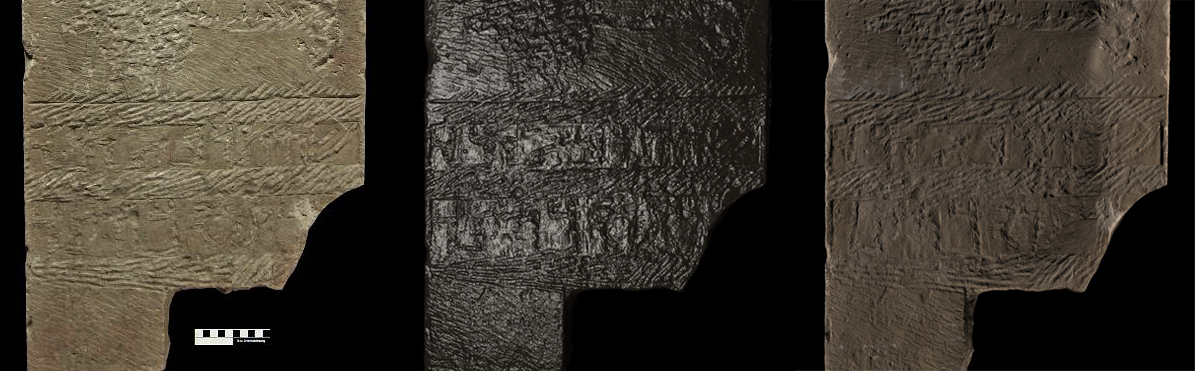
\includegraphics[width=0.85\textwidth]{bilder/rti_TA01029}
  \end{center}
  \caption{Ausschnitt der Rückseite der Grabstele TA 1029 mit reichsaramäischer Inschrift des Verstorbenen (Tayma, Saudi-Arabien). Links ein Foto. In der Mitte der gleiche Ausschnitt als RTI mit 'Specular Enhancement', rechts mit 'Static Multi Light'. (Foto: Mirco Cusin; RTI: Martina Trognitz, Max Haibt; DAI-Orient-Abteilung)}
\end{figure} 

\subparagraph{Polynomial Texture Map}
Ein Polynomial Texture Map (PTM) ist eine Repräsentationsform von Bildern mit Hilfe von Funktionen, statt einzelner Farbwerte. Im Gegensatz zu Rastergrafiken werden für die einzelnen Pixel von PTMs nicht nur feste Farbwerte gespeichert, sondern zusätzlich eine Funktion, die mit Hilfe der Parameter $l_u$ und $l_v$ die Leuchtdichte der Oberfläche berechnet. Die Leuchtdichte bestimmt wie das menschliche Auge eine Oberfläche wahrnimmt, also ob sie besonders hell, dunkel, spiegelnd oder matt erscheint.

%lu und lv noch einmal kontrollieren, so ganz kann das gerade nicht stimmen, was im ersten satz steht
Die Parameter $l_u$ und $l_v$ spezifizieren, wo sich eine punktförmige Lichtquelle befindet. Wird die Lichtquelle bewegt, ändern sich die Parameter und somit auch der errechnete Farbwert für den jeweiligen Pixel. Somit kann ein PTM simulieren, wie ein Objekt bei wechselnder Beleuchtungsrichtung aussieht.

Ganz vereinfacht lässt sich das Prinzip hinter RTI in der untenstehenden Abbildung visualisieren. Für jeden Punkt einer dreidimensionalen Oberfläche kann eine Normale bestimmt werden. An dieser Normale wird einfallendes Licht im gleichen Winkel reflektiert (Reflexionsgesetz). Da die Kamera sich in einer festen Position befindet, die Richtung aus der das Licht kommt ebenfalls bekannt ist und es einen Bilderstapel mit unterschiedlichen Lichtpositionen gibt, kann für jeden Bildpunkt eine Oberflächennormale berechnet werden. Wird die fertige RTI-Datei betrachtet und die Beleuchtung geändert, können die angezeigten Farbwerte der einzelnen Punkte anhand des gespeicherten Farbwertes, der errechneten Normalen und dem Einfallswinkel berechnet und ausgegeben werden.

\begin{figure}[!hpt]
  \begin{center}
    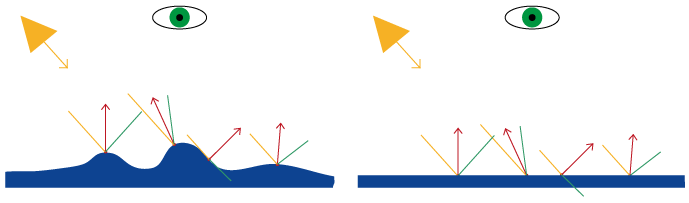
\includegraphics[width=0.9\textwidth]{bilder/rti_ptmAbstrakt}
  \end{center}
  \caption{Rechts sind auf einer dreidimensionalen Oberfläche für vier Punkte die Normalen (rot) eingezeichnet, an denen einfallendes Licht (gelb) reflektiert wird (grün). Links ist diese Obefläche als PTM dargestellt, in dem für die Punkte jeweils die Oberflächennormalen gespeichert sind. So entsteht ein optischer 3D-Effekt, der an sich aber nicht in der Datei hinterlegt ist.}
\end{figure}

\begin{wrapfigure}{r}{0.435\textwidth}
  \begin{center} \vspace{-0.6cm}
    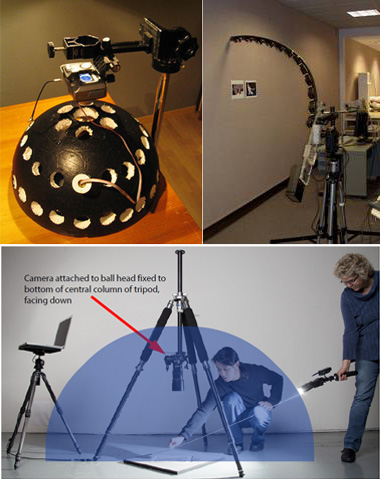
\includegraphics[width=0.435\textwidth]{bilder/rti_aufnahme}
  \end{center}
  \caption{Oben links eine Kuppel für RTI-Aufnahmen. Rechts ein gebogener Arm, der um das Objekt rotiert wird. Unten ist in den Aufbau von CHI eine imaginäre Kuppel projiziert. (Hewlett-Packard-Laboratories und CHI)}
\end{wrapfigure} 
\subparagraph{Aufnahmemethoden}
Das Grundprinzip für RTI-Aufnahmen besteht in der immer gleich bleibenden Position der Kamera in Bezug auf das Objekt und der wechselnden Position der Lichtquelle. Bei der Lichtquelle muss der Abstand zu dem Objekt immer der gleiche sein, um eine konstante Lichtintensität zu gewährleisten, und zusammen betrachtet sollten die jeweiligen Positionen so gewählt werden, dass sie gleichmäßig um das Objekt herum verteilt sind. Für die Positionierung der Lichtquellen wurden unterschiedliche Methoden und Ausrüstungsteile entwickelt, die in der nebenstehenden Abbildung zusammengefasst dargestellt sind.

Bei der Aufnahme mit einer Kuppel (engl. \emph{dome}) wird eine Kuppel so über das Objekt platziert, dass dieses in der Mitte liegt. Die Kamera wird ebenfalls mittig der Kuppel direkt über dem Objekt platziert. An der Kuppel können mehrere Lichtquellen, wie etwa LEDs befestigt sein, wobei bei jedem Bild jeweils nur eine eingeschaltet wird. Es gibt auch Kuppeln, die statt fest eingebauter Lichtquellen nur Markierungen für eine manuelle Platzierung der Lichtquelle haben. Die Position der Lichtquellen ergeben sich aus den Abmessungen der Kuppel und müssen in dem Programm eingetragen werden.

Eine vereinfachte Form der Kuppel sind gebogene Arme, mit daran befestigten Lichtquellen, wie etwa externe Blitzgeräte. Dieser Arm kann um das Objekt herum rotiert werden, so dass am Ende der Aufnahme eine kuppelförmige Verteilung der Lichter erzielt wird. Auch hier kann die Position der Lichtquellen aus den Abmessungen des Armes und dem Rotationswinkel berechnet werden.

Eine sehr flexible Methode, Highlight-RTI, wurde von Cultural Heritage Imaging entwickelt. Hierfür wird nur ein Blitzgerät (oder eine andere Lichtquelle) benötigt, an dem eine Schnur befestigt wird, mit deren Hilfe man das Gerät so ausrichten kann, dass der Abstand immer gleich ist und das Licht auch direkt auf das Objekt gerichtet ist. Auf diese Weise kann man sich an einer imaginären Kuppel entlang orientieren. Um die Position der Lichtquelle errechnen zu können, wird neben das Objekt eine schwarz glänzende Kugel platziert, die auch auf jedem Bild zu sehen sein muss. Aus den Reflexionspunkten des Lichtes an der Kugel kann das Programm dann die Richtung, aus der das Licht kommt, berechnen.


\paragraph{Praxis} In diesem Abschnitt werden Programme vorgestellt, mit denen RTI-Daten erstellt und betrachtet werden können.

\subparagraph{Erstellung von RTI-Daten}
Für die Aufnahme und Erstellung von RTI-Daten gibt es zwei frei verfügbare Programme. Das eine ist das \emph{PTM Fitter Programm}, welches an den Hewlett-Packard-Laboratories entwickelt wurde und zugleich auch das erste Programm ist, dass diese Art von Daten erstellen konnte. Es kann auf allen gängigen Betriebssystemen verwendet werden. Das zweite Programm, \emph{RTIBuilder}, stammt von CHI und ist für Windows und Mac verfügbar. CHI stellt weitere Materialien zur Erstellung von RTI-Daten zur Verfügung und deren Webangebot dient als zentrale Anlaufstelle für alles rund um RTI. Sie bieten ebenfalls ein Forum für aktive Anwender an.

\begin{flushleft}
	RTIBuilder: \urllist{http://culturalheritageimaging.org/What_We_Offer/Downloads/Process/index.html}
	Weiteres Material von CHI: \urllist{http://culturalheritageimaging.org/What_We_Offer/Downloads/}
	PTM Fitter Program: \urllist{http://www.hpl.hp.com/research/ptm/downloads/download.html}
\end{flushleft}
	
	
\subparagraph{Ansicht von RTI-Daten}
RTI-Daten können nur mit speziellen Viewer-Programmen betrachtet werden. Von den Hewlett-Packard-Laboratories gibt es die frei verfügbare \emph{PTM Viewer Application}, die auf Windows, Mac und Linux verwendet werden kann. Das Team von CHI bietet den \emph{RTIViewer} an, der ebenfalls frei verfügbar ist und auf Windows und Mac läuft. Er bietet erweiterte Funktionalitäten, wie beispielsweise die Annotation von Dateien.

Für eine Präsentation der Daten auf Webseiten kann der \emph{WebRTIViewer} empfohlen werden, der an dem Visual Computing Laboratory von CNR-ISTI in Pisa entwickelt wurde.

\begin{flushleft}
	PTM Viewer Application: \urllist{http://www.hpl.hp.com/research/ptm/downloads/download.html}
	RTIViewer: \urllist{http://culturalheritageimaging.org/What_We_Offer/Downloads/View/index.html}
	WebRTIViewer: \urllist{http://vcg.isti.cnr.it/rti/webviewer.php}
\end{flushleft}


%##############################################################
\paragraph{Quellen}
\begin{flushleft}
Cultural Heritage Imaging: \urllist{http://culturalheritageimaging.org/}

Hewlett-Packard-Laboratories, PTM: \urllist{http://www.hpl.hp.com/research/ptm/}

S. Duffy -- P. Bryan -- G. Earl -- G. Beale -- H. Pagi -- E. Kotouala, Multi-light Imaging for Heritage Applications (2013) \urllist{https://www.historicengland.org.uk/images-books/publications/multi-light-imaging-heritage-applications/}

T. Malzbender -- D. Gelb -- H. Wolters, Polynomial Texture Maps, in: Proceedings of ACM Siggraph 2001 (2001) \urllist{http://www.hpl.hp.com/research/ptm/papers/ptm.pdf}

\quelltyp{Formatspezifikationen}
PTM: \urllist{http://www.hpl.hp.com/research/ptm/downloads/PtmFormat12.pdf}
RTI: \urllist{http://forums.culturalheritageimaging.org/index.php?app=core&module=attach&section=attach&attach_id=81}

\quelltyp{Tools und Programme}
	RTIBuilder: \urllist{http://culturalheritageimaging.org/What_We_Offer/Downloads/Process/index.html}
	Weiteres Material von CHI: \urllist{http://culturalheritageimaging.org/What_We_Offer/Downloads/}
	PTM Fitter Program: \urllist{http://www.hpl.hp.com/research/ptm/downloads/download.html}
	PTM Viewer Application: \urllist{http://www.hpl.hp.com/research/ptm/downloads/download.html}
	RTIViewer: \urllist{http://culturalheritageimaging.org/What_We_Offer/Downloads/View/index.html}
	WebRTIViewer: \urllist{http://vcg.isti.cnr.it/rti/webviewer.php}
\end{flushleft}


\newpage
\section{Satellitenmessungen}%%Ursprünglich: Satellitenbilder und subsubsection
\abschnittsautor{S. Reinhold}
	%
% Satellitenmessungen
%
Bitte beachten Sie, dass die Inhalte dieses Abschnittes den Inhalten des IT-Leitfadens des DAIs von 2011 entsprechen.
\begin{center}
\tib{\rule{0.9\textwidth}{0.2mm}}\vspace{3mm}
\end{center}

\paragraph{Einsatz von Hard- und Software in der Praxis}
Auf allgemeiner Ebene sind momentan die unter GoogleEarth einsehbaren Satellitenbilder eine gute Alternative zu kommerziellen Satellitenbildern. Die bei GoogleEarth verwandten Bilder stammen aus verschiedenen Quellen und haben eine unterschiedliche Auflösung. Diese schwankt von 30-15m pro Pixel im Fall der auf Landsat-Aufnahmen basierenden Grundbilder bis zu einer Auflösung von etwa 1m pro Pixel bei Detailausschnitten. Diese Bilder stammen vom Satelliten Quickbird und werden laufend in GoogleEarth integriert. Es lohnt sich daher immer wieder die interessierende Region anzuschauen.

Eine Übersicht über die Quickbird-Aufnahmen sowie den Zeitpunkt der Aufnahme lässt sich unter Layers/DigitalGlobe Coverage im GoogleEarth Menü abrufen.

GoogleEarth hat den Nachteil, dass die Bilder nur in einer verhältnismäßig schlechten Auflösung abgespeichert werden können und sie nicht georeferenziert sind. Eine Lösung ist ein Upgrade auf GoogleEarthPlus. Dieses kostet 20\$ pro Jahr und erlaubt es, eine bessere Auflösung abzuspeichern und GPS-Daten sowie geographische Positionen können aus .CSV-Dateien importiert werden.

Für die Nutzung von georeferenzierten Satellitenbildern besteht die Möglichkeit, Bilder der Landsat Satelliten 4,5 und 7 im Internet frei zu laden. Die Daten des Satelliten Landsat ETM+ stammen aus dem Jahr 2000. Diejenigen von Landsat TM aus den 1990'er Jahren und die Bilder von Landsat MMS aus dem Zeitraum von 1972-1978.

BILD Aus: Eurimage Products and Services Guide

Um Bilder zu laden steuert man auf der Homepage landsat.org unter dem link 'Search for imagery' die freien LandsatOrtho Daten an. Mit dem dort vorgegebenen Path-Row Finder kann man die entsprechenden Angaben zur interessierenden Region über ein interaktives Kartenmodul ermitteln. Wichtig ist es dazu den Popublocker (Internetexplorer: Extra/Popupblocker; Firefox: Extras-Einstellungen-Inhalt/Pop-up-Fenster blockieren) zu deaktivieren. Wichtig ist auch im Suchmodus die Kästchen WRS I und WRS II anzukreuzen und refresh map zu aktivieren. Nur so lassen sich dann mit dem Informations-Tool die entsprechenden Flugbahndaten ermitteln. Eine alternative Suchmöglichkeit bietet sich unter: \url{http://landsat.usgs.gov/tools_wrs-2_shapefile.php}. Dort sind ESRI-shp files herunter zu laden, die ebenfalls Path/Row Informationen enthalten.

Hat man die Angaben lassen sich bei \url{http://www.landsat.org/ortho/} die entsprechenden Daten ansteuern und kopieren. Die gezippten Daten müssen dann entzippt werden und man erhält verschiedene Datensätze im Format Geo-Tiff. Diese sind georeferenziert im System WGS 1984.

Die Auflösung der Landsat Bilder ist unterschiedlich und liegt bei 30m bzw. 15m per Pixel.

BILD Aus: Eurimage Products and Services Guide

Für detailliertere Satellitenbilder mit hoher Auflösung stehen momentan nur kommerzielle Anbieter zur Verfügung. Dort können georeferenzierte Bilder mit einer Auflösung bis unter 1m pro Pixel erworben werden. Die folgende Tabelle gibt einen Überblick über die vorhandenen Systeme und die Quellen, über die Bildausschnitte und Preisinformationen zu erhalten sind.

\paragraph{Fotografische Sensoren}
\begin{center}
	\begin{tabular}{l p{0.3\textwidth} p{0.5\textwidth}}
		\toprule
		Satelliten & Beschreibung & Internet-Quelle \\ \midrule
		CORONA & Satellitenaufnahmen aus den 1960er und frühen 1970er Jahren der amerikanischen Spionagesatelliten CORONA, LANYARD und ARGON. CORONA Bilder der Missionen KH4 und 6 haben eine Auflösung von 2-3m. Es empfiehlt sich die Angaben in den Missionsdokumentationen zu lesen. Und Bilder in 7 Micron scannen zu lassen. Nicht georeferenziert! & Allgemeine Angaben finden sich unter: \url{http://edc.usgs.gov/products/satellite/declass1.html#description} Bildauswahl unter: \url{http://edcsns17.cr.usgs.gov/EarthExplorer/} dort finden sich die CORONA Bilder unter der Angabe "`declassified images"'. Preis (2007): 30\$ pro Filmstreifen (die DVD ist jedoch recht teuer) \url{http://edcsns17.cr.usgs.gov/helpdocs/prices.html#CORONA}\\
		KFA-1000 & Der russische Spionagesatellit KFA-1000 hat eine Auflösung von 1.5-3m. Die Bilder Stammen aus den 1990er Jahren. Nicht georeferenziert! & Übersichtskarten und Bildauswahl sind erhältlich über \url{http://www.sovinformsputnik.com/}\\
		 	\bottomrule    
	\end{tabular}
\end{center}


\paragraph{Digitale Sensoren}
\begin{center}
	\begin{tabular}{l p{0.3\textwidth} p{0.5\textwidth}}
		\toprule
		Satelliten & Beschreibung & Internet-Quelle \\ \midrule
		LANDSAT & Amerikanische Multispektral-Satelliten, die seit 1972 aktiv sind. Die LANDSATs 1-3 hatten einen Multispektral Sensor (MSS) mit einer Auflösung von 80m. Die LANDSATs 4 and 5 haben MSS und Themaic Mapper (TM) Sensoren mit einer Auflösung von 30 oder 15m. & Übersicht bei \url{http://landsat.org} Kommerzielle Anbieter sind u.a. \url{http://www.eurimage.com/index.html} oder \url{http://www.digitalglobe.com/} Preise (2007) ab 250 EURO \url{http://www.eurimage.com/products/docs/eurimage_price_list.pdf} \\
		SPOT & SPOT. Französische Satelliten mit Multispektral (XS) Sensoren und einer Auflösung von 20m bis 10m. & Bilder und Preisangaben bei \url{http://www.spotimage.fr/html/_.php}\\
		IKONOS 2 & Satellit mit hochauflösenden Kameras, die Graustufen- und Farbbilder aufnehmen. Jedes Bild bildet eine Fläche von mindestens 11 x 11 km mit einer Auflösung von bis zu 0,82m ab. Es können auch Flächen von 60 x 60 km in einem Überflug aufgenommen werden können. & Bilder und Preisangaben bei \url{http://www.euspaceimaging.com/} Preis ca. 30\$ pro qkm\\
		QuickBird & QuickBird 2 ist ein kommerzieller Satellit zur Erdbeobachtung. Er wird von DigitalGlobe betrieben. Er hat eine Auflösung von 0,6m. Die Detailbilder in GoogleEarth sind Quickbirdaufnahmen seit 2001. & Bilder und Preisangaben bei \url{http://www.digitalglobe.com/} oder \url{http://www.eurimage.com/index.html} Preis 16-41 \$ pro qkm (mindestens 272 qkm)\\
		 	\bottomrule    
	\end{tabular}
\end{center}


\paragraph{Quellen}
\begin{flushleft}
\url{http://www.dainst.org/medien/de/Nasca-BMBF_Programm.pdf}

David L. Kennedy, Declassified satellite photographs and archaeology in the Middle East: case studies from Turkey. Antiquity 72, Nr. 277 1998, 553-561.

Graham Philip/Daniel Donoghue/Anthony Beck/N. Galiatsatos, CORONA satellite photography: an archaeological application from the Middle East. Antiquity 76, Nr. 291 2002, 109-118.

Jason Ur, CORONA satellite photography and ancient road networks: A Northern Mesopotamina case study. Antiquity 77, Nr. 295 2003, 102-105.

Wouter Gheyle/Raf Trommelmans/Jean Bourgeois/Rudi Goosens/Ignace Bourgeois/Alain De Wulf/Tom Wilkens, Evaluation CORONA: A case study in the Altai Republic (South Siberia). Antiquity 78, Nr. 300 2004, 391-403.

M. Altaweel, The use of ASTER satellite imagery in archaeological contexts. Archaeological Prospection 12, 2005, 151-166.

K.N. Wilkinson/Anthony Beck/Graham Philip, Satellite imagery as a resource in the prospection for archaeological sites in central Syria. Geoarchaeology 21, 2003, 735-750.

Anthony Beck/Graham Philip/Maamun Abdulkarim/Daniel Donoghue, Evaluation of CORONA and IKONOS high resolution satellite imagery for archaeological prospection in western Syria. Antiquity 81, Nr. 311 2007, 176-190.
\end{flushleft}





%%%%%%%%%%%%%%%%%%%%%
%% Alte Gliederung %%
%%%%%%%%%%%%%%%%%%%%%
%\section{Anthropologoie}
%\subsection{Genetik (Genotyp)}
%\subsection{Morphologie und Metrik (Phänotyp)}
%\subsection{Physiologie (Ökotyp)}
%\subsection{Verhaltensforschung (Ethotyp)}

%\section{Archäobotanik}
%\subsection{Makroreste}
%\subsection{Pollenanalyse (Palynologie)}

%\section{Archäozoologie}

%\section{Ausgrabung}
%\section{Bauforschung}
%\subsection{Bauaufnahme}

%\section{Datierung}
%\subsection{Andere Methoden}
%\subsection{C14-Datierung}
%\subsection{Dendrochronologie}
%\subsection{OSL/TL-Datierung}
%\subsection{Uran-Ungleichgewichtsmethoden}

%\section{Geoarchäologie}
%\subsection{Biomarker}
%\subsection{Bodenuntersuchungen}
%\subsection{Geologische Untersuchungen}
%\subsection{Geomorphologie}
%\subsection{Sedimentuntersuchungen (Bohrkerne)}

%(Geodatenanalyse)
%\subsection{Geocodierung und Geoparsing}
%\subsection{Geomorphometrie}
%\subsection{Visualisierung und Kartierung}


%\section{Geophysik}
%\subsection{Geoelektrik}
%\subsection{Geomagnetik}
%\subsection{Georadar}

%\section{Materialaufnahme}
%\subsection{3D-Scanning} (DFG Digitalisierung hat auch einen Abschnitt dazu)
%\subsection{Nahbereichsphotogrammetrie}
%\subsection{RTI}

%\section{Materialwissenschaftliche Archäometrie}
%\subsection{Anorganische Materialien}
%\subsubsection{Gesteine}
%\subsubsection{Metalle}
%\subsubsection{Silikatische Materialien}

%\subsection{Methoden}
%\subsubsection{Bildgebende Verfahren}
%\subsubsection{Chemische Verfahren}
%\subsubsection{Isotopenuntersuchung}
%\subsubsection{Physikalische Verfahren}

%\subsection{Organische Materialien}
%
%\section{Numismatik}
%\section{Oberflächenbegehung (Survey)}
%\section{Statistische Daten}

%\section{Textwissenschaften und Schriftzeugnisse}
%%In this section we cover the main kinds of text providing for each of them an overview of problems, existing standards, existing tools and recommended best practices. Also for each type of text we suggest possible workflows with different levels of depth of text encoding. The first step will be always creating a metadata catalog for the texts we are dealing with, etc.
%%
%%\begin{itemize}
%%	\item goal: to provide a set of recommendations and best practices to follow when encoding textual sources.
%%	\item Also we want to put the currently available standards in the context of the specific problems and perspectives of the disciplines that IANUS aims to cater for, such as for instance Archaeology.
%%	\item The way texts have been treated to date has lead to a perceivable dichotomy between the communities of those who deal with texts and those who deal with objects, which often are also text-bearing objects.
%%	\item more than just saying which standards should be used, in this document we want to state clearly what are the problems and challenges we are faced with when encoding textual sources electronically
%%	\item identifying the intended use of data and the target user community
%%	\item open challenges are:
%%	\begin{itemize}
%%		\item theoretical problems related to texts
%%		\begin{itemize}
%%			\item encoding text and the problem of interpretation
%%			\item function/role of the editor, shift from print to digital era
%%		\end{itemize}	
%%	\end{itemize}	
%%	\begin{itemize}
%%		\item interoperability of encoding formats
%%		\begin{itemize}
%%			\item interoperability between texts
%%			\item interoperability between tools that analyse and manipulate texts
%%		\end{itemize}	
%%	\end{itemize}	
%%\end{itemize}
%
%\subsection{Sprachen und Zeichensysteme}
%%Matteo Romanello
%%Markus Schnöpf -> siehe Vortrag 2014 DCSB
%
%%Auszeichnungssprachen vertiefen; SGML, XML; sowie TEI ausführen
%%Texttechnologie?
%
%
%%the choice of an encoding format is not merely a technical one, but has both theoretical and practical implications and consequences. These decisions are inevitable, therefore it is important to be aware of such implications in order to make an informed decision.
%%
%%Character encoding; maybe OCR; 
%
%\subsubsection{Ägyptisch}
%\subsubsection{Akkadisch}
%\subsubsection{Aramäisch}
%\subsubsection{Griechisch}
%\subsubsection{Hebräisch}
%\subsubsection{Hethitisch}
%\subsubsection{Latein}
%\subsubsection{Sumerisch}
%
%\subsection{Antike Objekte mit Texten}
%\subsubsection{Gefäße}
%\subsubsection{Inschriften}
%%EpiDoc guidelines (\url{http://www.stoa.org/epidoc/gl/latest/})
%
%%list of projects using EpiDoc: \url{http://www.stoa.org/epidoc/gl/latest/app-bibliography.html}
%
%%EAGLE project: \url{http://www.eagle-network.eu/}
%
%\subsubsection{Manuskripte}
%%	\url{http://www.digipal.eu/}
	%
%%	\url{http://www.homermultitext.org/}
%
%%	\url{http://homermultitext.blogspot.de/}
	%
%\subsubsection{Papyri}
%%	\url{http://www.papyri.info/}
	%
%\subsubsection{Siegel}
%\subsubsection{Tontafeln}
%
%\subsection{Literarische Schriftquellen}
%%	Digital Latin Library: \url{http://www.apaclassics.org/index.php/research/digital_latin_library_project}
%
%%	Classical Works Knowledge Base:	\url{http://www.cwkb.org/}
%
%%	Perseus Catalog:	\url{http://catalog.perseus.org/}
%
%\subsection{Veröffentlichung und Archivierung}
%%Mit Rücksicht auf Werkzeuge und Plattformen
%%\begin{itemize}
%%	\item SoSOL for papyri and inscriptions (Philologist  perseid, as presented at DH2012)
%%	\item Arachne's TEI/OCR editor
%%	\item Open Journal System (OJS) for journals
%%	\item CTS repositories and CITE suite
%%\end{itemize}
%
%\subsubsection{Wissenschaftliche Editionen}
%%\begin{itemize}
%%	\item the term scholarly edition is intentionally rather general: the idea is not to limit this category to any discipline in particular. 
%%	\item	a set of general problems related to scholarly editions are to be identified
%%	\item then there are specific kinds of texts which challenge the print-based model of scholarly edition, for instance fragmentary texts
%%	\item \url{http://wiki.tei-c.org/index.php/Critical_Apparatus_Workgroup}
%%	\item \url{http://www.i-d-e.de/aktivitaeten/reviews/kriterien-version-1}
%%\end{itemize}
%
%\subsubsection{Schnittstellen zu Textsammlungen}
%%\begin{itemize}
%%	\item OAI-PMH as sort of a minimum to expose a collection of resources
%%	\item then there exist more sophisticated protocols to access text collections such as the CTS protocol
%%\end{itemize}
%\subsubsection{Kollaborative Arbeitsumgebungen}
%%emphasis on platforms and licenses that allow the users to contribute to the texts and to improve them (OCR corrections, levels of annotation, etc.)
%\subsubsection{Publikation}
%%XML Print (\url{https://sites.google.com/a/budabe.eu/xmlprint_de/home}) DFG-funded project, developed by UTrier, and related to TextGrid. Goal is to make easier to produce (high quality/precision) print output out of XML/TEI encoded texts.
%\subsubsection{Lizenzierung}
%%\begin{itemize}
%%	\item as soon as data are published online, a license must be attached to them. Possibly an open one. 
%%	\item Put the open licensing in the context of crowdsourcing and the virtuous cycle of open access; new projects and initiatives can be built on top of openly licensed materials
%%\end{itemize}